
\documentclass{article} % For LaTeX2e
\usepackage{iclr2027_conference,times}

% Optional math commands from https://github.com/goodfeli/dlbook_notation.
\input{math_commands.tex}

\usepackage{hyperref}
\usepackage{url}
\usepackage{booktabs}
\usepackage{array}
\usepackage{graphicx}
\usepackage{pifont}
\usepackage{float}
\usepackage[table]{xcolor}
\usepackage{comment}
\usepackage{wrapfig}
\usepackage{capt-of}

% Enable colored links and set specific color mappings
\hypersetup{
    colorlinks=true,      % False: bordered boxes; True: colored text
    citecolor=blue,       % Change citation link colors to blue
    linkcolor=black,      % Keep internal section/equation links black
    urlcolor=black        % Keep external URL links black
}

\title{PhysicsLENS: Diagnosing Physical Property Blindness in Video Generation Models}

% Authors must not appear in the submitted version. They should be hidden
% as long as the \iclrfinalcopy macro remains commented out below.
% Non-anonymous submissions will be rejected without review.

\author{Antiquus S.~Hippocampus, Natalia Cerebro \& Amelie P. Amygdale \thanks{ Use footnote for providing further information
about author (webpage, alternative address)---\emph{not} for acknowledging
funding agencies.  Funding acknowledgements go at the end of the paper.} \\
Department of Computer Science\\
Cranberry-Lemon University\\
Pittsburgh, PA 15213, USA \\
\texttt{\{hippo,brain,jen\}@cs.cranberry-lemon.edu} \\
\And
Ji Q. Ren \& Yevgeny LeNet \\
Department of Computational Neuroscience \\
University of the Witwatersrand \\
Joburg, South Africa \\
\texttt{\{robot,net\}@wits.ac.za} \\
\AND
Coauthor \\
Affiliation \\
Address \\
\texttt{email}
}

% The \author macro works with any number of authors. There are two commands
% used to separate the names and addresses of multiple authors: \And and \AND.
%
% Using \And between authors leaves it to \LaTeX{} to determine where to break
% the lines. Using \AND forces a linebreak at that point. So, if \LaTeX{}
% puts 3 of 4 authors names on the first line, and the last on the second
% line, try using \AND instead of \And before the third author name.
\definecolor{Everyone}{RGB}{0, 150, 136}  % teal
\definecolor{Rans}{RGB}{228, 26, 28}      % red
\definecolor{Jiqing}{RGB}{152, 78, 163} % purple
\definecolor{Xinyuan}{RGB}{77, 175, 74}   % green
\definecolor{Aditya}{RGB}{255, 127, 0}    % orange
\definecolor{Som}{RGB}{166, 86, 40}       % brown
\definecolor{Isaiah}{RGB}{172, 145, 21}    % mustard yellow

\newcommand{\Jiqing}[1]{\textcolor{Jiqing}{\textbf{@Jiqing:} #1}}
\newcommand{\Everyone}[1]{\textcolor{Everyone}{\textbf{@Everyone:} #1}}
\newcommand{\Rans}[1]{\textcolor{Rans}{\textbf{@Rans:} #1}}
\newcommand{\Xinyuan}[1]{\textcolor{Xinyuan}{\textbf{@Xinyuan:} #1}}
\newcommand{\Aditya}[1]{\textcolor{Aditya}{\textbf{@Aditya:} #1}}
\newcommand{\Som}[1]{\textcolor{Som}{\textbf{Som:} #1}}
\newcommand{\Isaiah}[1]{\textcolor{Isaiah}{\textbf{@Isaiah:} #1}}

\newcommand{\fix}{\marginpar{FIX}}
\newcommand{\new}{\marginpar{NEW}}

%\iclrfinalcopy % Uncomment for camera-ready version, but NOT for submission.
\begin{document}


\maketitle

\begin{abstract}
% Reliable video world models could provide scalable environments for robot learning, planning, and evaluation, but their usefulness depends on predicting physically consistent video. Visually consistent video alone is not sufficient. The generated videos can appear convincing while depicting physically impossible interactions. Moreover, not all properties governing an interaction are observable from appearance. For example, a large box in the video may be empty and light or filled and heavy, leading to different responses to the same applied force. A reliable world model must therefore use observable evidence when informative and incorporate specified physical properties when visual evidence is insufficient. <Then connect with current benchmark...>

% Existing benchmarks typically return plausibility scores, offering little insight into whether a model genuinely reasons about the physical properties governing a scene or merely reproduces motion correlated with visual appearance.

Reliable video world models could provide scalable predictive environments for robot learning, planning, and evaluation. However, robot videos can violate physical principles and complete tasks through physically implausible behavior, limiting their reliability for robot learning and planning. 
Current video-generation benchmarks exclude physics that are inherently hidden by visuals (eg: weight, viscosity, friction). Due to this, video models are evaluated on the fidelity of physics- not the underlying accuracy of physics. 
We introduce PhysicsLENS, a dataset and benchmark for evaluating plausibility of physical properties grounded in robotics. PhysicsLENS uses matched scenario pairs that hold the same conditioning frame and action, while varying underlying physics in the scene description. Scenarios are curated from public robot video sources and annotated across seven physical domains: collision, gravity, momentum, friction, deformation, fluid, and causality. We evaluate across four video generation models, producing over 400 human-annotated labels. 
Results show a consistent accuracy gap between observable and unobservable conditions, indicating that models rely on visual appearance rather than grounded text-specified properties.

% , and that VLM-based diagnosis further struggles with compound violations spanning multiple constraints in a single clip.

\end{abstract}

\section{Introduction}
% With the rapid progress of egocentric robotics, the need for video training data has risen exponentially. Current video generation models face a wide gap in accuracy, and widely vary in quality depending on the model and content premise. Video generation models finetuned to a specific task are not enough to address the data deficit found across real-life scenarios- which often involve complicated physics, multiple object interactions, and unseen physics reactions. Prior physics benchmarks have established that video generation models struggle with physical consistency broadly, but most report this as a single aggregate score, leaving open where physical understanding specifically breaks down: whether a model fails at physics in general, or only when the governing property cannot be read directly from the frame. To address this, we introduce PhysicsLENS, a benchmark and dataset that varies observability as its own axis, together with a diagnostic pipeline we test as an automated approximation of human judgment.  
Video world models could provide scalable predictive environments for robot learning, planning, and evaluation. By generating diverse interactions without repeated real-world data collection, they may expose robots to rare events, unfamiliar objects, and changing physical conditions. However, scaling the quantity of generated data is useful only if the resulting videos provide physically reliable supervision. A video may look realistic and show a robot completing its task while violating friction, momentum, object permanence, or other physical constraints. Such failures limit the value of generated videos as representations of how actions affect the physical world.

Existing video-generation benchmarks only partially measure this reliability. Most emphasize visual quality, temporal consistency, or the plausibility of motion visible in a generated video. These criteria can identify obvious artifacts, but they do not determine whether a model correctly grounds the physical properties specified in its conditioning input. Properties such as weight, friction, viscosity, and deformability may not be observable from a single image. Consequently, visually identical scenes can require different outcomes: a robot should interact differently with a heavy object than with a light one, or with a slippery surface than with a rough one. A model can therefore generate a plausible video while producing behavior that is physically incorrect for the stated condition.

We introduce \textbf{PhysicsLENS}, a dataset and benchmark for evaluating physical plausibility and physical-property grounding in robot video generation. PhysicsLENS uses matched scenarios that hold the conditioning frame, task, and visual scene constant while varying a text-specified physical property. This design distinguishes whether a generated video merely appears physically plausible from whether it responds correctly to the specified condition. The benchmark covers seven physical domains relevant to robotic interaction: collision, gravity, momentum, friction, deformation, fluid dynamics, and causality. Scenarios are curated from public robot-video sources to capture diverse embodiments and interactions without requiring large-scale collection of new demonstrations.

\begin{figure*}
  \centering
  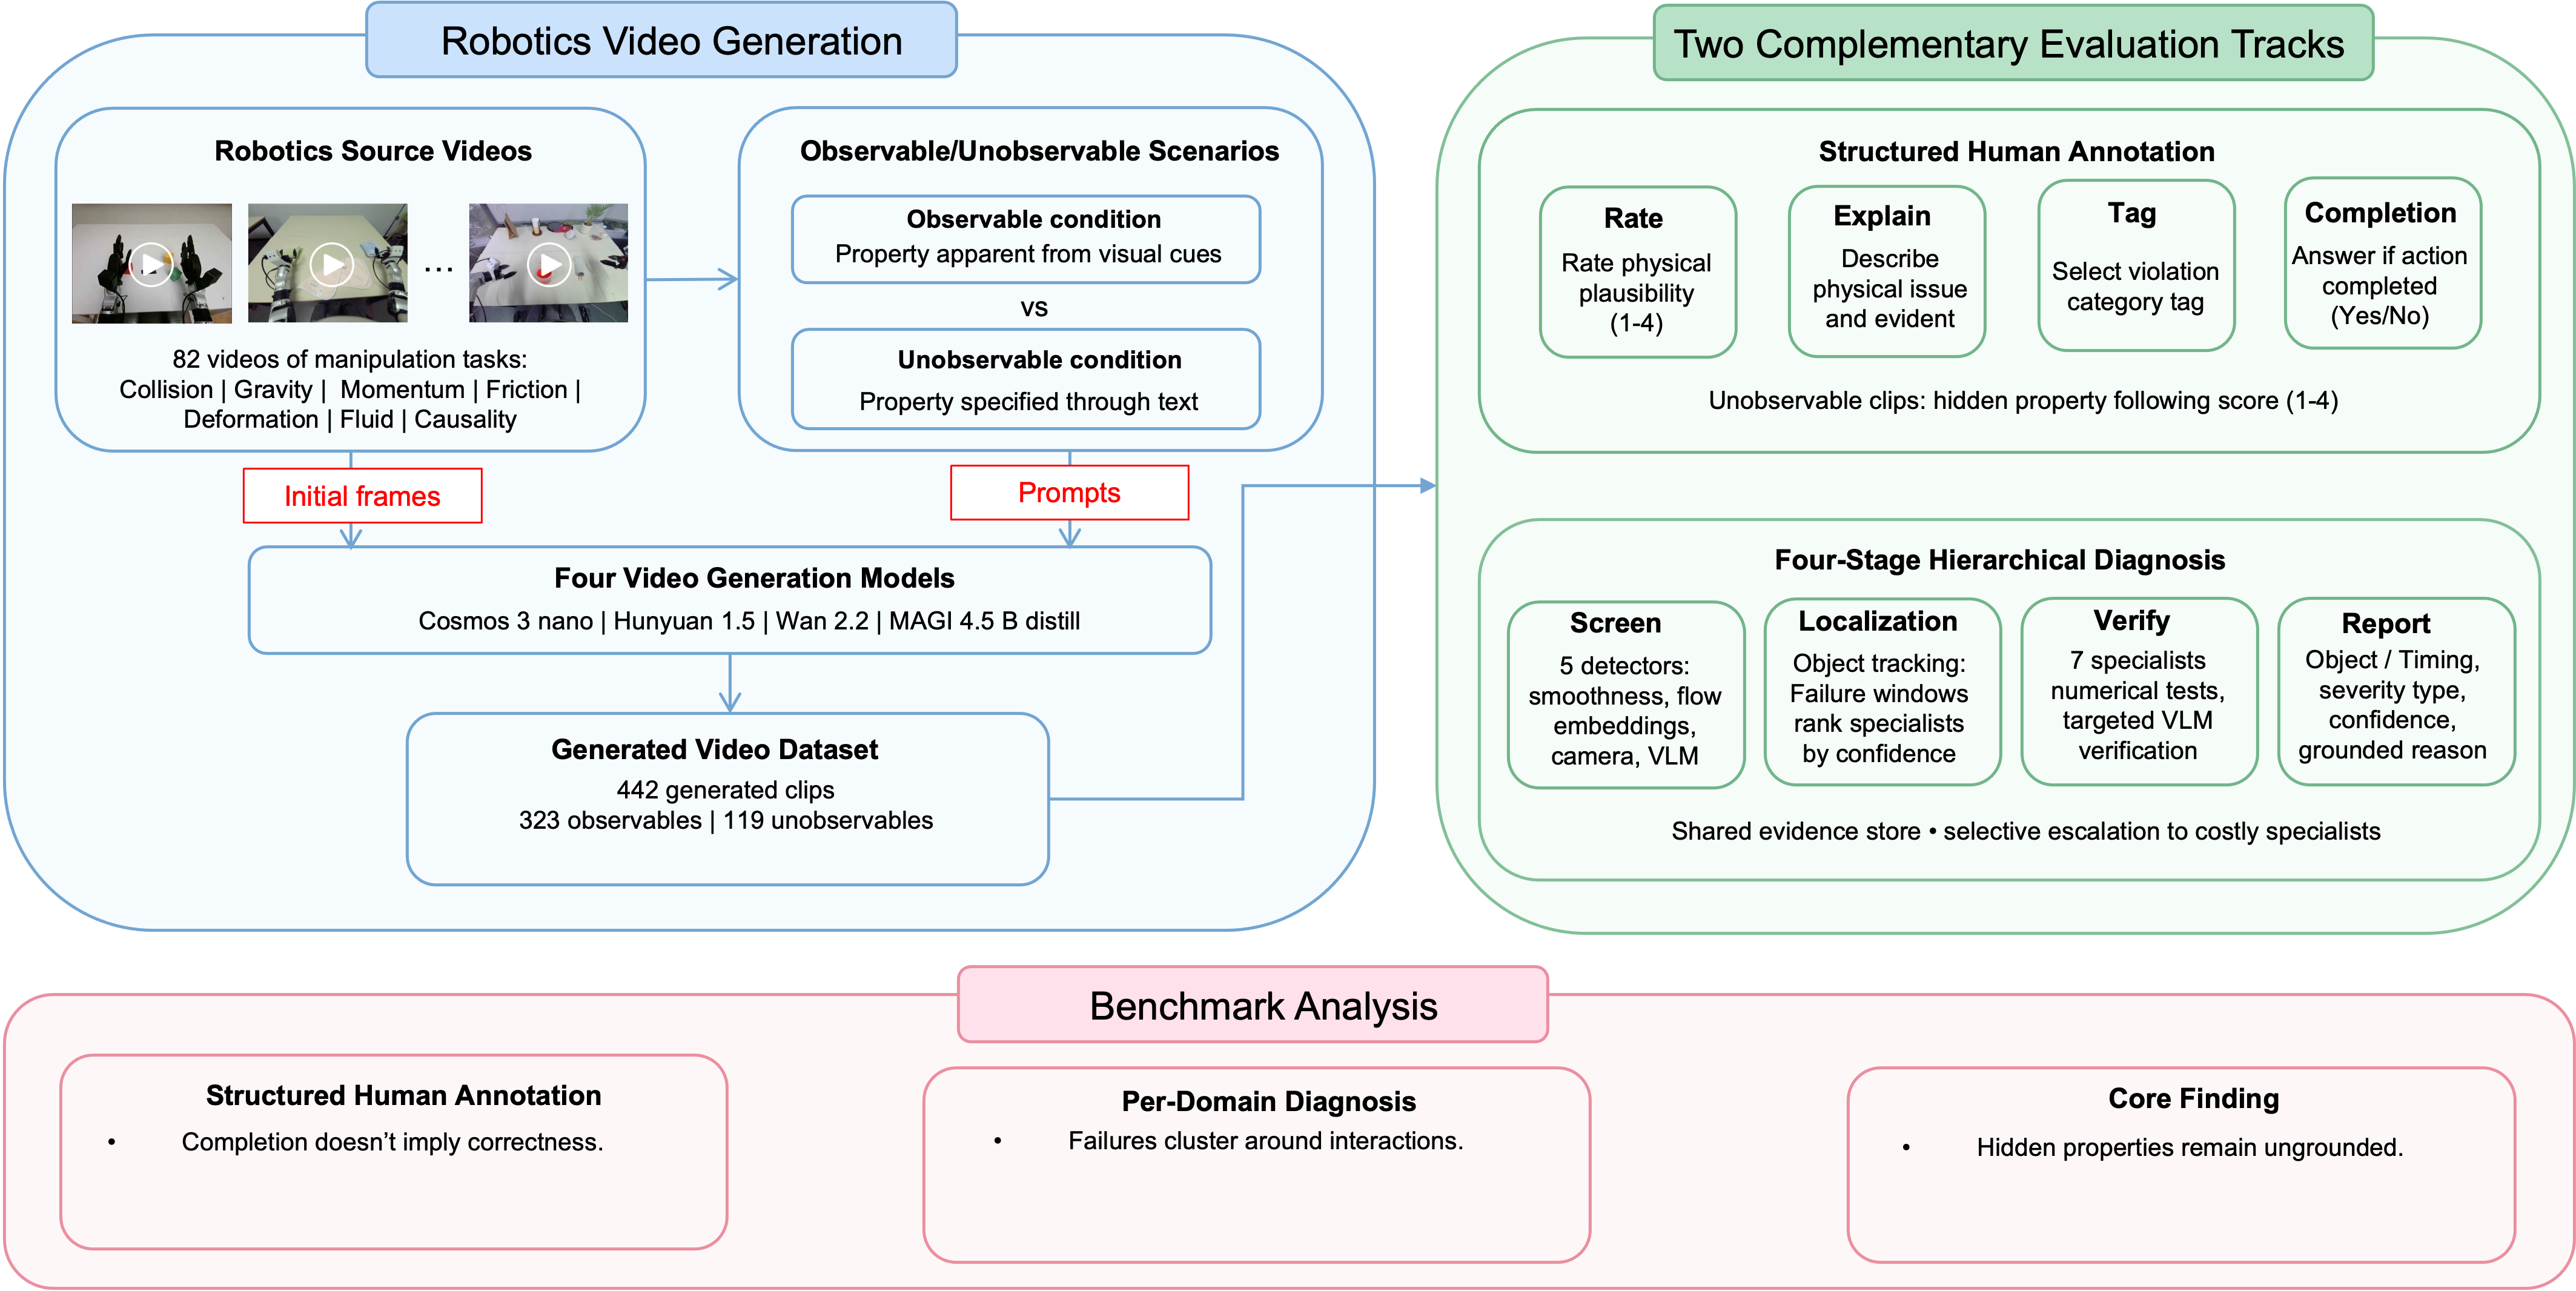
\includegraphics[width=\linewidth]{fig/Diagram.png}
  \caption{The workflow of PhysicsLENS.}
  \label{fig:systemdiagram}
\end{figure*}


% Accurate evaluation also presents a cost--quality trade-off. Human assessment can detect subtle physical violations but is expensive to apply at scale, whereas a single automated plausibility score is inexpensive but provides limited diagnostic information. PhysicsLENS addresses this trade-off through a multi-stage agentic evaluation procedure that decomposes assessment into task completion, physical plausibility, and consistency with the specified physical condition. This structure supports scalable screening while providing interpretable diagnoses of how and why a generated video fails.

Our contributions are:
\begin{enumerate}
\item We introduce PhysicsLENS, a robotics-focused benchmark covering seven physical domains and distinguishing physical plausibility from physical-property grounding.
\item We construct matched scenarios that preserve visual context while varying text-specified physical conditions, including properties that cannot be inferred from appearance alone.
\item We present a multi-stage agentic evaluation procedure and benchmark four video-generation models with more than 400 human judgments, revealing a consistent gap between observable and unobservable physical conditions.
\end{enumerate}
% Contributions of this work:
% \begin{enumerate}
%     \item \textbf{An observability axis for physical property grounding.} We introduce the first benchmark to evaluate whether video generation models can correctly apply a physical property specified only in text when that property is not visually apparent in the conditioning frame. We introduce matched scenario pairs that hold the conditioning frame and action constant while varying only whether the governing physical property is visually apparent or specified exclusively through text, testing whether models perform physical reasoning over stated properties or generate motion from appearance alone. We find how strongly a model followed a stated hidden property does not correlate with how plausible annotators rated the clip, showing that plausibility scores alone cannot reveal whether a model is grounding what it was told. This axis is distinct from Physion++ \citep{tung2023physionevaluatingphysicalscene}, which infers latent properties from observed interaction rather than explicit specification, and T2V-CompBench \citep{sun2025t2vcompbenchcomprehensivebenchmarkcompositional}, which evaluates only visually observable properties.

%     \item \textbf{A physics-annotated robotics benchmark revealing domain coverage gaps.} We curate a benchmark of AI-generated robot manipulation scenarios generated from public robotics video sources and annotate each scenario with its failed physical domain. This annotation process surfaces a systematic imbalance in existing robotics data: scenarios involving solid-object contact and manipulation are abundant, while scenarios involving fluid interaction are comparatively scarce, and phenomena outside these categories are largely absent. Rather than treating physical plausibility as a single aggregate score, our per-domain annotation enables evaluation and diagnosis to be reported separately for each physical domain.

%     \item \textbf{Testing automated diagnosis against human judgment.} Alongside human annotation, we implement a four-stage pipeline --- screening, localization, specialist evaluation, and reporting --- that produces a diagnosis rather than a scalar plausibility score, and test whether it can approximate human judgment without access to ground-truth expected outcomes. We report where automated diagnosis agrees with human annotators and where it does not, rather than presenting the pipeline as a validated substitute for human scoring.

%     % \item We demonstrate how insights from this large-scale benchmarking can be used to guide model improvement, enabling targeted enhancements in performance based on identified failure modes and capability gaps.
% \end{enumerate}

\section{Related Work}
% \subsection{Video Generation and World Models}
% Recent text- and image-conditioned video models produce increasingly compelling clips, with representative open-weight systems including VideoCrafter2, CogVideoX, Wan \citep{wan2025wanopenadvancedlargescale}, HunyuanVideo \citep{wu2025hunyuanvideo15technicalreport}, and LTX-Video, alongside proprietary systems such as Sora, Veo, Kling, Seedance, and Runway. Newer generations have improved visual fidelity, temporal coherence, prompt adherence, and controllability, while increasingly supporting multiple conditioning modalities, longer sequences, and synchronized audio. In parallel with these advances in content generation, a growing line of research is adapting video-generative architectures for world modeling, where models predict how an observed environment may evolve over time, potentially conditioned on agent actions. Cosmos \citep{agarwal2025cosmos}, for example, is explicitly designed as a world foundation model platform for robotics and autonomous driving, while autoregressive systems such as MAGI-1 \citep{ai2025magi1autoregressivevideogeneration} support causal, streaming video generation as an early step toward general-purpose simulators of the physical world.

% Despite these advances, generated videos still contain objects that float, accelerate inconsistently, or interact implausibly \citep{le2025gravity}. Visual realism is also a poor predictor of physical correctness \citep{motamed2026physicsiq}. Controlled experiments further suggest that strong in-distribution video prediction does not necessarily imply the acquisition of general physical laws: \citet{kang2025howfar} found that video models often rely on case-based similarities and fail to extrapolate reliably to out-of-distribution physical configurations. Detecting such failures before generated video is used for downstream training remains difficult and often depends on costly human review.

\newcommand{\lensyes}{\ding{51}}
\newcommand{\lensno}{\ding{55}}
\newcommand{\lensunknown}{?}

\begin{table*}[t]
\centering
\scriptsize
\setlength{\tabcolsep}{3.5pt}
\renewcommand{\arraystretch}{0.96}
\caption{
Comparison of physics benchmarks and video critics.
Ref.-free requires no paired real-world recording;
Obs.\ axis tests prompt-specified properties not inferable
from the initial frame.
\lensyes: supported; \lensno: unsupported.
}
\label{tab:related}

\begin{tabular}{@{}l*{6}{c}@{}}
    \toprule
    Method
    & Physics
    & Robotics
    & Human
    & Ref.-free
    & Localized
    & Obs.\ axis \\
    \midrule

    \multicolumn{7}{@{}l}{\emph{Physics benchmarks and evaluators}} \\[-2pt]
    VideoPhy-2~\citep{bansal2026videophy}
    & \lensyes & \lensno & \lensyes & \lensyes & \lensno & \lensno \\
    PhyGenBench~\citep{meng2024phygenbench}
    & \lensyes & \lensno & \lensno & \lensyes & \lensno & \lensno \\
    Morpheus~\citep{zhang2025morpheus}
    & \lensyes & \lensno & \lensno & \lensno & \lensno & \lensno \\
    Physics-IQ~\citep{motamed2026physicsiq}
    & \lensyes & \lensno & \lensno & \lensno & \lensno & \lensno \\
    NewtonRewards~\citep{le2025gravity}
    & \lensyes & \lensno & \lensno & \lensyes & \lensno & \lensno \\
    GeoPhys~\citep{internò2026geophysgeometryphysicalplausibility}
    & \lensyes & \lensno & \lensno & \lensyes & \lensyes & \lensno \\

    \midrule
    \multicolumn{7}{@{}l}{\emph{Robotics evaluators}} \\[-2pt]
    RoboGaze~\citep{nguyen2026robogazeevaluatingrobotworld}
    & \lensyes & \lensyes & \lensyes & \lensyes & \lensyes & \lensno \\
    RBench~\citep{RBench_deng2026rethinkingvideogenerationmodel}
    & \lensyes & \lensyes & \lensyes & \lensyes & \lensno & \lensno \\
    RoboWM-Bench~\citep{jiang2026robowmbenchbenchmarkevaluatingworld}
    & \lensyes & \lensyes & \lensno & \lensno & \lensyes & \lensno \\

    \midrule
    \multicolumn{7}{@{}l}{\emph{Latent properties and attribute binding}} \\[-2pt]
    Physion++~\citep{tung2023physionevaluatingphysicalscene}
    & \lensyes & \lensno & \lensyes & \lensno & \lensno & \lensno \\
    T2V-CompBench~\citep{sun2025t2vcompbenchcomprehensivebenchmarkcompositional}
    & \lensno & \lensno & \lensno & \lensyes & \lensyes & \lensno \\

    \midrule
    \multicolumn{7}{@{}l}{\emph{VLM reasoning and diagnostics}} \\[-2pt]
    Cosmos-Reason1~\citep{nvidia2025cosmosreason}
    & \lensyes & \lensyes & \lensno & \lensyes & \lensyes & \lensno \\
    QuantiPhy~\citep{puyin2026quantiphy}
    & \lensyes & \lensno & \lensyes & \lensyes & \lensno & \lensno \\
    MASS~\citep{wu2026mass}
    & \lensyes & \lensno & \lensyes & \lensyes & \lensyes & \lensno \\

    \midrule
    \rowcolor{orange!15}
    \textbf{PhysicsLENS}
    & \lensyes & \lensyes & \lensyes
    & \lensyes & \lensyes & \lensyes \\
    \bottomrule
\end{tabular}

\end{table*}


\paragraph{Physics evaluation of generated video.}
Visual quality does not guarantee physical correctness: generated videos can contain implausible interactions despite appearing realistic \citep{le2025gravity,motamed2026physicsiq}, and strong in-distribution prediction need not imply generalization to unfamiliar physical configurations \citep{kang2025howfar}. Distributional metrics such as FVD \citep{unterthiner2018towards} and broader evaluation suites such as VBench \citep{huang2024vbench} measure distributional similarity and perceptual properties rather than directly testing compliance with physical laws. Recent benchmarks address physics more explicitly. VideoPhy separates semantic adherence from physical commonsense and introduces VideoCon-Physics as an automatic evaluator \citep{bansal2025videophy}; VideoPhy-2 extends this framework to more complex, action-centric scenarios with finer-grained physical-rule annotations \citep{bansal2026videophy}. PhyGenBench evaluates prompts covering 27 physical laws through a staged VLM--LLM pipeline \citep{meng2024phygenbench}, while PhyWorldBench and WorldModelBench provide additional benchmarks for evaluating video-based world models \citep{gu2026phyworldbenchcomprehensiveevaluationphysical, li2025worldmodelbenchjudgingvideogeneration}. Morpheus compares generations against controlled physical experiments and conservation laws \citep{zhang2025morpheus}, Physics-IQ evaluates predicted continuations against recorded real-world outcomes \citep{motamed2026physicsiq}, and NewtonRewards extracts measurable motion quantities to define verifiable rewards for constant-acceleration primitives \citep{le2025gravity}. Together, these efforts document physical inconsistencies across generation settings and model families. However, benchmarking generators under predefined conditions does not necessarily establish whether a model follows a particular prompt-specified physical property. Aggregate scores also need not identify when a violation occurs, which object is responsible, or which constraint is violated.

\paragraph{Robotics world-model evaluators.}
A related line of work evaluates physical plausibility in robot-manipulation videos. RoboGaze \citep{nguyen2026robogazeevaluatingrobotworld} combines task-scene grounding, dimension-specific specialists, and critic-based verification to produce temporally localized glitch reports under a robotics-specific taxonomy. RBench \citep{RBench_deng2026rethinkingvideogenerationmodel} and RoboWM-Bench \citep{jiang2026robowmbenchbenchmarkevaluatingworld} likewise evaluate manipulation-centric world models, with the latter converting generated behavior into action sequences validated in simulation. These approaches situate physical plausibility within broader evaluations that also consider task adherence, subject consistency, or embodiment fidelity. They provide useful precedents for structured evaluation, but their manipulation-centric protocols do not explicitly isolate whether a governing physical property is apparent in the conditioning image or supplied only through language.

\paragraph{Hidden properties and attribute binding.}
Two further lines of work inform this observability distinction. Physion++ \citep{tung2023physionevaluatingphysicalscene} evaluates prediction in scenarios requiring the inference of latent mechanical properties---including mass, friction, elasticity, and deformability---from observed interactions. Its findings indicate that predictive accuracy alone does not establish human-like inference of these properties. Our setting differs in both task and available information: rather than inferring an unstated property from an observation period, the generator must translate an explicitly stated property into subsequent dynamics. T2V-CompBench \citep{sun2025t2vcompbenchcomprehensivebenchmarkcompositional} evaluates the binding of prompt-specified attributes to objects and identifies dynamic attribute binding as a persistent challenge. Its focus on visually verifiable attributes, such as color, shape, and motion direction, differs from testing mechanical properties that have no distinguishing signature in the initial frame but become evident through their effects on motion. PhysicsLENS makes this distinction an explicit evaluation axis through matched scenarios that control scene and action while contrasting visually apparent and text-only property information. Its scoring separates physical plausibility from adherence to the stated property. We find that these measures dissociate: adherence to hidden properties shows little relationship to how plausible the resulting clips appear. Plausibility alone therefore cannot establish whether a generator grounds the physical properties specified in its input.

\paragraph{VLM judges and structured evaluators.}
Multimodal models offer a promising basis for automated physical assessment. Cosmos-Reason1, for example, is post-trained for physical commonsense and embodied reasoning across spatial, temporal, and dynamic relationships \citep{nvidia2025cosmosreason}. Nevertheless, producing a score or answering a question differs from diagnosing a violation, which requires temporal localization, object attribution, and identification of the relevant constraint. PQSG and Physion-Eval are additional related efforts in physical assessment \citep{pothiraj2026physicsquestionscenegraph, zhang2026physionevalevaluatingphysicalrealism}, alongside approaches that examine or strengthen the evidence supporting multimodal judgments. QuantiPhy shows that plausible verbal explanations can coexist with inaccurate estimates of velocity and acceleration \citep{puyin2026quantiphy}, while MASS augments VLM reasoning with depth-based spatial representations, object grounding, and motion tracking \citep{wu2026mass}. GeoPhys provides a particularly important caution: in its physics-violation detection setting, VLM judges including GPT-4o and Gemini perform near chance, as does the video-representation model V-JEPA 2, whereas a training-free score computed from frozen image-encoder feature trajectories achieves stronger detection performance without a VLM judge \citep{internò2026geophysgeometryphysicalplausibility}. These results, together with documented limitations in fine-grained motion analysis and temporal grounding \citep{hong2025motionbench,wang2025grounded}, motivate an evidence-grounded, staged diagnostic design rather than reliance on a single holistic judgment. They do not, however, establish that staging alone resolves evaluator unreliability. We therefore test this directly by comparing our automated diagnostic pipeline against structured human annotations on the same clips.

% 2.3 — the machinery our pipeline builds on; hand off to Section 3.
% Argue: VLMs/MLLMs enable temporal reasoning and model-as-critic judging, but haven't been specialized for fine-grained physics diagnosis.
% \subsection{Vision-Language Models for Video Understanding and Critique}
\begin{comment}
Recent multimodal models show promising physical-reasoning capabilities. Cosmos-Reason1, for example, is post-trained for physical commonsense and embodied reasoning across spatial, temporal, and dynamic relationships \citep{nvidia2025cosmosreason}. 
Such models are commonly used as scorers or question-answering systems, whereas diagnosis also requires temporal localization, object attribution, and identification of the violated constraint.
Recent work has attempted to improve this grounding. 
QuantiPhy shows that VLMs can produce plausible verbal explanations while remaining inaccurate when estimating numerical properties such as velocity and acceleration \cite{puyin2026quantiphy}. 
MASS supplements VLM reasoning with depth-based spatial representations, object grounding, and motion tracking, further demonstrating the importance of explicit spatiotemporal evidence for physical analysis \cite{wu2026mass}.
The unreliability of VLM-based judgment on this task is stark: on physics-violation detection, GPT-4o, Gemini, and V-JEPA 2 all perform near chance, while GeoPhys, a training-free score computed directly from frozen image-encoder feature trajectories with no VLM component at all, achieves state-of-the-art detection \citep{internò2026geophysgeometryphysicalplausibility}.
Because current models remain unreliable at fine-grained motion analysis and temporal grounding \citep{hong2025motionbench,wang2025grounded}, it is unclear whether a staged VLM pipeline can reliably approximate human judgment of physical plausibility at all; we test this directly, comparing an automated diagnostic pipeline against structured human annotation on the same clips.
\end{comment}

\section{PhysicsLENS Benchmark}
\subsection{Observable vs Unobservable Physical Properties}
\label{sec:observability}
A generated video is conditioned on two sources of information: the visual content of the initial frame and the text prompt describing the scene and the action to follow. For most physical properties relevant to a manipulation scenario---an object's mass, a surface's friction, a fluid's viscosity---these two sources are typically redundant in real-world footage: a large object usually looks heavy, a wet surface usually looks slippery. This redundancy means that a model could, in principle, generate physically plausible motion by relying on visual appearance alone, without any genuine grounding of the physical property in question.

We introduce an experimental axis that breaks this redundancy. For each scenario we distinguish between two conditions:

\begin{description}
    \item[Observable] The physical property governing the outcome has a visual correlate in the conditioning frame. A robot arm is positioned to squeeze a round, beige toy on a table; the toy appears soft, made of a flexible material such as foam, with a smooth surface likely to compress easily under pressure.
    \item[Unobservable] In the matched unobservable condition, the conditioning image remains unchanged. The scene description instead specifies that the toy is extremely resistant to deformation and retains its shape under pressure. This condition tests whether the generated interaction follows the stated property, which cannot be reliably inferred from the image alone.
\end{description}

This distinction isolates a question that no prior physics evaluation protocol asks directly: does a video generation model perform genuine physical reasoning over the properties described to it, or does it generate motion primarily as a function of visual appearance, treating the text prompt as auxiliary rather than governing information? A model that merely pattern-matches appearance to motion should perform well on observable scenarios, where the visual cue and the correct outcome are aligned, but should fail on unobservable scenarios, where no such cue exists and the outcome can only be inferred by correctly grounding the stated property.

\paragraph{Matched pair construction.} To isolate observability as the sole experimental variable, we construct unobservable scenarios as paired variants of existing observable scenarios rather than as independent frames. Each pair shares an identical conditioning frame and an identical action description; the only difference between the two prompts is the scene description, which in the observable condition describes a visually apparent property and in the unobservable condition instead states a hidden property in its place. Holding the frame and action constant across the pair ensures that any difference in generated physics is attributable to observability alone, rather than to confounds such as scene complexity, action difficulty, or frame quality.

\begin{figure}[t]
    \centering
    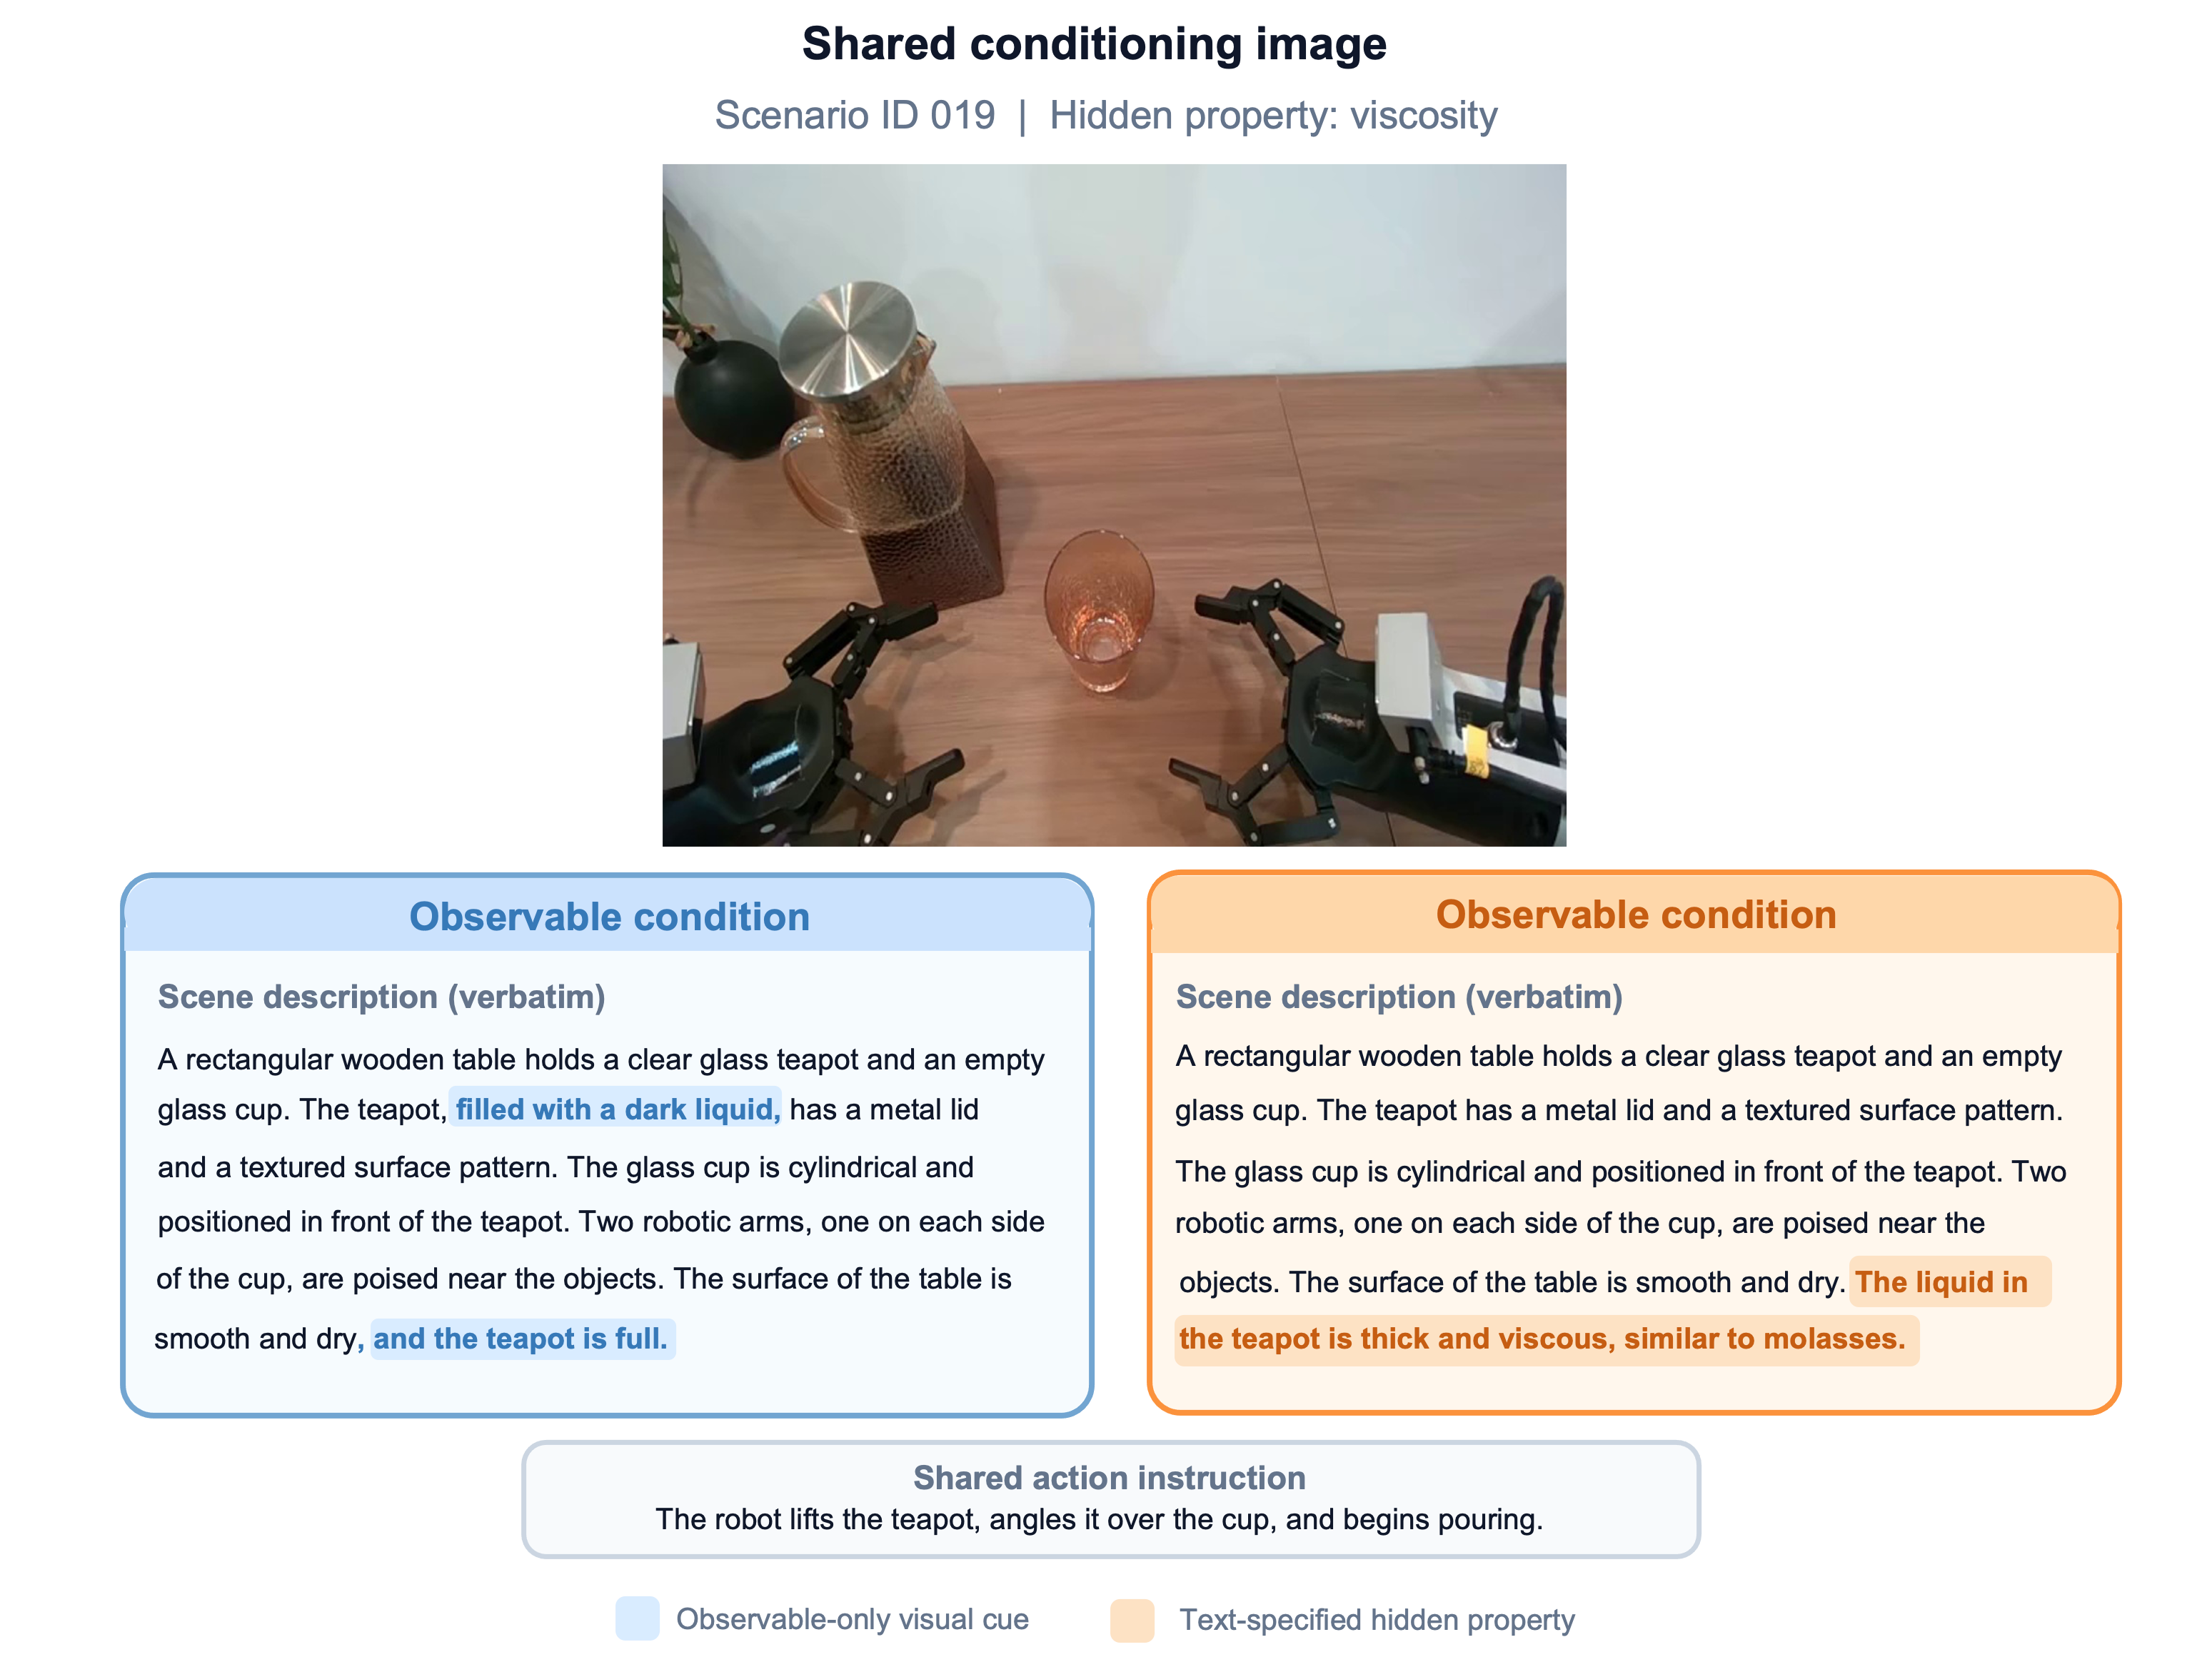
\includegraphics[width=\linewidth]{fig/fig_conditioning_image_prompts.png}
    \caption{Construction of a matched prompt pair.
    Both conditions use the same conditioning frame and
    action instruction. Highlighted text identifies the
    change in the scene description, including the physical
    property specified in the unobservable condition.
    The intervention changes the textual physical
    specification, not the visual content of the frame.}
    \label{fig:matched-prompt-construction}
\end{figure}

\paragraph{The hidden-property mechanism.} Each unobservable scenario is annotated with two additional fields beyond those used for observable scenarios: a \texttt{hidden\_property}, naming the category of physical property not obvious from the frame, and a \texttt{hidden\_property\_value}, the specific plain-language value stated in the prompt (e.g., ``extremely resistant to deformation''). We use four hidden-property categories, one per task group: viscosity for pouring scenarios, surface condition for wiping scenarios, elasticity for deformable-object scenarios, and mass for pushing scenarios. The hidden property is stated in the scene description, which conditions the video generator, while the corresponding \texttt{expected\_outcome} is withheld from the generator entirely and used only for downstream human annotations, consistent with our broader design principle that the pipeline must operate without access to ground truth (\S\ref{sec:pipeline}).

\paragraph{Failure mode under test.} For each unobservable scenario we additionally record a \texttt{failure\_signature}: a description of the specific, observable way a model would fail if it disregarded the text-stated property and instead defaulted to a generic or appearance-driven physical response. For example, given a prompt stating that a visually ordinary box is filled with dense material, the corresponding failure signature is that the box moves with the same speed and resistance as an unmarked, unweighted object---indicating the model ignored the stated mass and generated motion based on the object's unremarkable appearance alone. We refer to this failure mode as \emph{appearance-property conflation}: a systematic reliance on visual appearance as a proxy for physical properties, even when those properties are explicitly and unambiguously specified in text. Section~\ref{sec:results-grounding} reports the extent to which this failure mode is present, and consistent, across the video generation models we evaluate.

\subsection{Physics Taxonomy and Domain Coverage}
\begin{wraptable}{r}{0.52\linewidth}
\vspace{-12pt}
\centering
\caption{Physics domain taxonomy used to inform scenario design and annotation.}
\label{tab:taxonomy}
\footnotesize
\setlength{\tabcolsep}{3.5pt}
\begin{tabular}{@{}p{1.8cm}>{\raggedright\arraybackslash}p{4.95cm}@{}}
\toprule
Domain & Representative scenario types \\
\midrule
Collision    & Grasping, placing, stacking, contact-dependent lifting \\
Friction     & Pushing, wiping, sliding along a surface \\
Momentum     & Object release, swinging, mass-dependent resistance \\
Fluid        & Pouring, transferring, absorbing liquid \\
Deformation  & Folding, squeezing, compressing, crumpling \\
Gravity      & Dropping, tipping, unsupported release \\
Causality    & Cross-cutting: effect must follow cause with no spontaneous state change \\
\bottomrule
\end{tabular}
\vspace{-10pt}
\end{wraptable}
Table~\ref{tab:taxonomy} lists seven physical domains --- collision,
friction, momentum, fluid, deformation, gravity, and causality ---
constructed from the physical dynamics that commonly arise in
robotic manipulation tasks generally, rather than derived from the
specific scenarios in this benchmark.

Causality is a cross-cutting exception: rather than a scenario type
of its own, it is evaluated across every scenario as a check that no
object appears, disappears, or changes state without a corresponding
physical cause. Scenarios in this benchmark were curated from public
robotics video sources without selecting for coverage of specific
domains; we do not report a per-scenario domain assignment or
per-domain scenario counts. This taxonomy informs scenario design
and the annotation rubric (\S\ref{sec:human-annotation}) rather than
functioning as a per-scenario label, and it precedes and is
independent of which scenarios were ultimately selected.

\subsection{Dataset Design}
PhysicsLENS contains 110 prompts: 80 observable scenarios and 30 unobservable scenarios constructed as matched variants of a subset of the observable set. In observable scenarios, the relevant physical condition is visually apparent; in unobservable scenarios, it is specified only in text. By holding the visual context and action constant, these pairs test whether a model follows the specified physics rather than defaulting to visual priors.
Starting frames were collected from public robotics videos, including Unitree G1 manipulation footage, and selected to depict clear robot--object interactions involving solids or liquids. General physics benchmarks~\citep{tung2023physionevaluatingphysicalscene,motamed2026physicsiq,meng2024phygenbench} do not involve embodied agents, while robotics-specific evaluators~\citep{nguyen2026robogaze,RBench_deng2026rethinkingvideogenerationmodel} typically inherit scenarios from existing demonstrations rather than constructing controlled variations of physical properties. To our knowledge, existing benchmarks do not explicitly compare visually observable properties with properties specified only through text.
Each conditioning image depicts the scene immediately before the target action. Images were standardized to $1280\times720$, and every prompt specifies a static camera to prevent camera motion from being mistaken for object motion. Scene and action descriptions were generated under a fixed schema and manually reviewed. We generate one video per prompt with each of four models---Wan 2.2, Cosmos, HunyuanVideo 1.5, and MAGI 4.5B Distill---yielding 440 videos. Appendix~\ref{app:dataset-details} provides the complete preprocessing and prompting procedure.

\subsection{Human Annotation Protocol}
\label{sec:human-annotation}
Each generated video is evaluated along three complementary dimensions: physical plausibility $P\in\{1,2,3,4\}$, binary action completion $A\in\{0,1\}$, and, for unobservable scenarios, hidden-property adherence $H\in\{1,2,3,4\}$. Annotators also provide a free-text diagnosis and select applicable physical-violation categories. We report the dimensions separately because a video may complete the requested action through implausible behavior or appear plausible while ignoring a text-specified property.

We report rating distributions, descriptive means, and action-completion proportions. For thresholded summaries, $P\geq3$ denotes mostly plausible or realistic behavior, while $H\geq3$ denotes that the specified property is mostly or fully followed. Each video received one annotation, so the data do not support an estimate of inter-annotator reliability; matched pairs were also not necessarily rated by the same annotator. The full rubrics, violation-label definitions, allocation procedure, and aggregation details appear in Appendix~\ref{app:annotation-details}.

\section{Multi-Stage Agentic Evaluation}
\subsection{Automated Diagnostic Pipeline}
\label{sec:pipeline}

Alongside human annotation, PhysicsLENS organizes automated
physical diagnosis into four stages: screening, localization,
specialist evaluation, and reporting. The pipeline is intended
to produce structured explanations of candidate violations
rather than only a scalar plausibility judgment.
Its components are evaluated against the human annotations
in Section~\ref{sec:results-tool}; automated outputs are not
used to compute the human results reported in this paper.

\begin{figure*}[t]
    \centering
    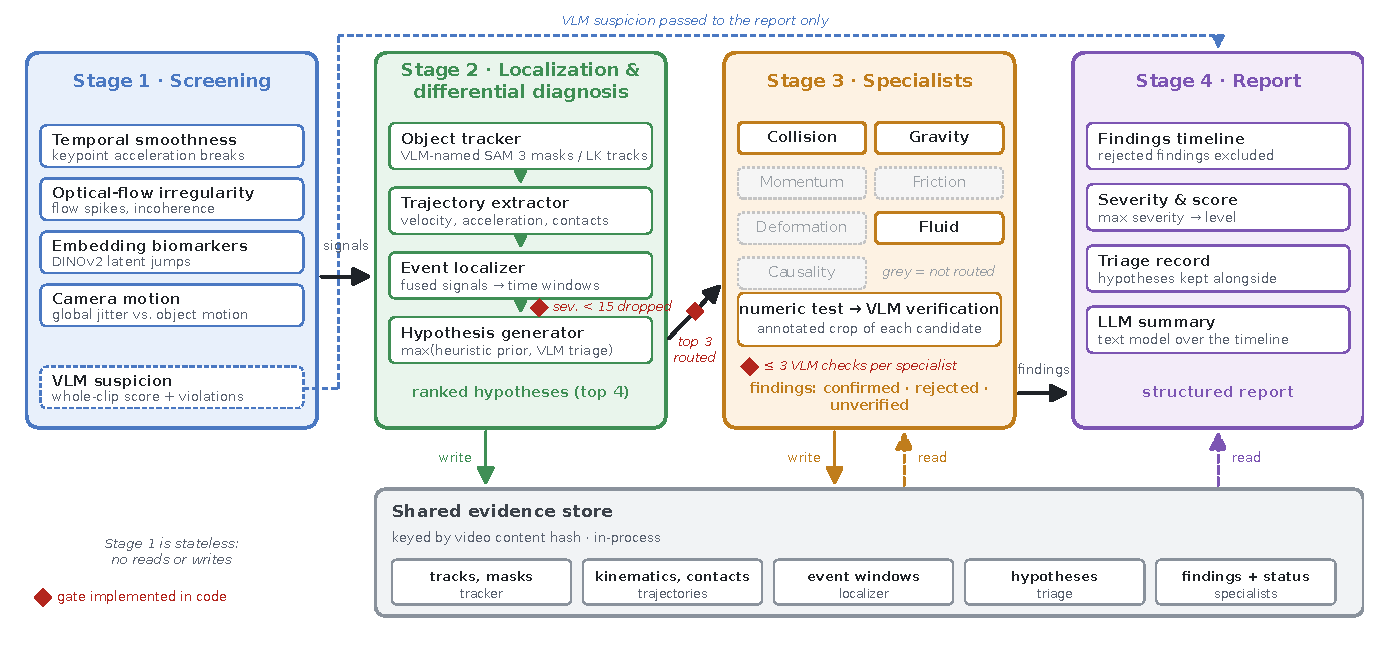
\includegraphics[width=\linewidth]{fig/pipeline.pdf}
    \caption{Evidence flow through the PhysicsLENS diagnostic pipeline, as
    implemented. Stage-1 detectors produce timestamped suspicion signals, which the
    orchestrator passes to the Stage-2 event localizer; the Stage-1 VLM suspicion
    score is passed only to the report. Stage~2 tracks VLM-named objects, extracts
    kinematics and contacts, localizes candidate events, and ranks constraint
    families by the maximum of a heuristic prior and a VLM triage score; the three
    highest-ranked families are routed to their specialists (grey: not routed, not
    run). Each specialist proposes violations numerically and verifies a bounded
    number of them with the VLM, labelling each finding confirmed, rejected, or
    unverified; the report excludes rejected findings. Stages~2 and 3 write to a
    shared evidence store keyed by the video's content hash, from which Stages~3
    and 4 read; Stage~1 is stateless. Red diamonds mark the gates present in the
    implementation. The diagram describes the architecture; its accuracy is
    evaluated in Section~\ref{sec:results-tool}.}
    \label{fig:pipeline-evidence-flow}
\end{figure*}

\paragraph{Screening.}
The screening stage examines the generated video and its
conditioning information to identify candidate physical
inconsistencies and relevant constraint families.
A screening flag is a candidate for further examination,
not a verified violation.

\paragraph{Localization.}
The localization stage associates candidate issues with
the relevant temporal interval and interacting objects.
Localization is intended to connect a diagnosis to
visible evidence, rather than leaving it as a
video-level assertion.

\paragraph{Specialist evaluation.}
Domain specialists assess candidate events against the
physical constraints summarized in
Table~\ref{tab:specialists}. Property-specific assessment
must use the stated physical condition, rather than
assuming that a visually familiar object has its
usual material properties. Specialist judgments must
also distinguish an observed inconsistency from
insufficient visual evidence.

\paragraph{Reporting.}
The reporting stage organizes the diagnostic findings
into a structured account of the implicated constraints,
relevant events, and supporting observations.
The stage descriptions specify the intended functional
roles; they do not establish diagnostic accuracy.

% IMPLEMENTATION DETAILS REQUIRED BEFORE SUBMISSION:
% Verify the paragraphs above against the actual implementation.
% Add the exact backend/checkpoint used at each stage;
% video decoding, temporal sampling, and image resolution;
% prompt templates and decoding settings;
% screening and specialist-routing rules;
% localization representation and temporal resolution;
% information passed between stages;
% specialist output schemas;
% aggregation and conflict-resolution rules;
% retry/failure handling and software version.
% Do not describe these choices as implemented until verified.

\Isaiah{Look at sec/method.tex to get deeper more specific info. Plan to put that in Supplementary}

\subsection{Domain-Specific Diagnostic Checks}
\label{sec:specialist-checks}

Table~\ref{tab:specialists} specifies the physical questions
associated with each specialist. These checks describe
the intended scope of diagnosis, not validated detector
capabilities. A single event may implicate multiple
constraint families.

\begin{table}[t]
    \centering
    \small
    \caption{Intended diagnostic scope of the seven
    PhysicsLENS specialists. Checks require visible evidence
    or an explicit property specification; they do not assume
    access to hidden forces, complete material parameters,
    or a reference outcome. Contact and Collision remain
    separate labels in the human annotation export.}
    \label{tab:specialists}
    \begin{tabular}{@{}p{0.16\linewidth}p{0.77\linewidth}@{}}
        \toprule
        Specialist & Diagnostic questions \\
        \midrule
        Collision &
        Do interactions respect object boundaries?
        Is apparent penetration inconsistent with the
        objects' rigidity, and is motion attributed to
        contact supported by visible interaction? \\

        Friction &
        Is sticking, slipping, or sliding consistent with
        the visible contact and any stated surface
        condition? Are changes in resistance supported
        by the interaction? \\

        Momentum &
        Are abrupt changes in translational or rotational
        motion supported by an interaction? Where mass
        is specified, does the video provide enough
        evidence to assess its consequences? \\

        Fluid &
        Is flow consistent with the visible container
        geometry and interaction? Are stated properties
        such as viscosity reflected in the observed
        flow, when the action exposes them? \\

        Deformation &
        Do changes in shape follow the interaction and
        any stated material properties? Are apparent
        shape changes physical deformation or
        unsupported morphing? \\

        Gravity &
        Is unsupported motion consistent with gravity,
        accounting for visible support and contact?
        Is apparent floating distinguishable from
        unresolved support or perspective? \\

        Causality &
        Do object appearances, disappearances, and
        state changes have visible or otherwise
        supported causes? Could an apparent
        discontinuity instead result from occlusion? \\
        \bottomrule
    \end{tabular}
\end{table}

\Isaiah{Complete once evals come through}
\subsection{Comparison with Human Judgments}
\label{sec:pipeline-human-comparison}

The human ratings provide a reference for agreement, not an
error-free physical ground truth; Section~\ref{sec:results-tool}
compares the pipeline's outputs with them. Physical plausibility
and hidden-property adherence are compared as ordinal ratings: we
report AUC for separating ratings 3--4 from 1--2, and linearly
weighted Cohen's $\kappa$ after mapping continuous scores onto the
1--4 scale by quantile matching. Hidden-property adherence is
compared only on unobservable scenarios. Action completion is
compared with AUC and Cohen's $\kappa$.

For violations, we report per-family AUC for \emph{detection}
(videos with the family versus videos with no recorded violation)
and \emph{attribution} (videos with the family versus videos with
a different violation). The annotators record Contact separately
from Collision; because the pipeline has a single collision
specialist, we merge Contact into Collision and state this wherever
family-level results are reported.

Confidence intervals are bootstrap intervals over videos. Every
choice fitted to the data---signal selection and orientation, and
the mapping from scores to ratings---uses five-fold
cross-validation grouped by scenario, so that records of the same
scenario stay together across models and conditions. One component
was not developed on disjoint data: the debiased judge prompt of
Section~\ref{sec:results-tool} was written after inspecting these
videos, and we therefore validate it on VideoPhy-2, a dataset it
was not designed on.


\subsection{Reference-Outcome-Free Diagnosis}
\label{sec:ground-truth-free}

The pipeline's design excludes access to
\texttt{expected\_outcome}, reference outcome videos, and
human evaluation labels during inference. Its permitted
evidence consists of the generated video and conditioning
information, including the initial image, requested action,
and any text-specified physical property.

The stated property is part of the model input and is
therefore available to the evaluator. This differs from
providing a reference description of how the generated
action should unfold. Human labels may be used afterward
to measure agreement, but must not be supplied to the
diagnostic stages.

This restriction supports evaluation when a reference
continuation is unavailable. It does not remove physical
ambiguity: forces, material parameters, occluded contacts,
and other relevant quantities may remain unknown.
A diagnosis must therefore be supported by the available
evidence and should allow an insufficient-evidence outcome
rather than treating every ambiguous interaction as a
physical violation.

% =====================================================================
% Section 5: Experimental Results (full section).
%   5.1  plausibility vs. grounding, human (RQ1)
%   5.2  observable vs. text-specified, human (RQ2)
%   5.3  failure cases (RQ3)
%   5.4  automated diagnosis (RQ4)            -- Som, with Aditya
% Tables in 5.3 are generated by backend/scripts/paper_tables.py;
% regenerate rather than hand-edit numbers. Self-contained: no \input.
% =====================================================================

\section{Experimental Results}
\label{sec:results}

This section presents results on the PhysicsLENS benchmark and evaluates its diagnostic pipeline through four research questions. RQ1--RQ3 are answered with human annotations, and RQ4 compares the pipeline against them. \textbf{RQ1:} Does high physical plausibility imply that a model followed a text-specified physical property (Sec.~\ref{sec:results-grounding})? \textbf{RQ2:} Does stating a property in text rather than showing it reduce physical plausibility (Sec.~\ref{sec:results-paired})? \textbf{RQ3:} What do individual failure cases reveal about the distinction between grounding and plausibility (Sec.~\ref{sec:results-cases})? \textbf{RQ4:} Can the PhysicsLENS pipeline approximate human judgments (Sec.~\ref{sec:results-tool})?

\subsection{RQ1: Does High Plausibility Imply Property Grounding?}
\label{sec:results-grounding}
A video can look physically realistic and still ignore the physics it was asked to show. Annotators rate each video's physical plausibility $P$ and, for unobservable videos, its adherence $H$ to the stated property, both on a 1--4 scale (Section~\ref{sec:human-annotation}): $P \geq 3$ means the video is mostly or fully physically realistic, and $H \leq 2$ means the stated property is mostly or completely ignored. Of the 119 unobservable videos, 47 are rated plausible ($P \geq 3$), yet 34 of these (72\%) ignore the stated property ($H \leq 2$). All four generators produce such videos (Table~\ref{tab:hidden-results}, Figure~\ref{fig:joint-ratings}). MAGI contributes 21 of the 34, but the pattern does not depend on it: without MAGI, 13 of the remaining 26 plausible videos (50\%) still ignore the property.

% Table 4 and Figure 4 side by side, top and bottom aligned: the plot's height
% is set to (table + its caption) - (figure caption), so both columns end together.
\newsavebox{\PLtab}\newsavebox{\PLcap}
\begin{figure}[t]
    \centering
    \sbox{\PLtab}{\begin{minipage}[t]{0.52\linewidth}
        \vspace{0pt}
        \centering
        \setlength{\abovecaptionskip}{0pt}
        \captionof{table}{Human evaluation on unobservable scenarios. $\bar{P}$, $\bar{H}$: mean plausibility and adherence (1--4). Compl.: completion rate.}
        \label{tab:hidden-results}
        \footnotesize
        \setlength{\tabcolsep}{2pt}
        \resizebox{\linewidth}{!}{%
        \begin{tabular}{@{}l r r r r r@{}}
            \toprule
            Model & $n$ & $\bar{P}$ & $\bar{H}$ & Compl. & $H{\le}2 \mid P{\ge}3$ \\
            \midrule
            HunyuanVideo 1.5  & 29 & 2.24 & 2.24 & 72.4\% & 5/13 (38.5\%) \\
            MAGI 4.5B distill & 30 & 3.10 & 1.10 &  6.7\% & 21/21 (100\%) \\
            Wan 2.2           & 30 & 1.53 & 1.90 & 40.0\% & 2/5 (40.0\%) \\
            Cosmos-nano 1     & 30 & 2.07 & 1.87 & 66.7\% & 6/8 (75.0\%) \\
            \bottomrule
        \end{tabular}}
    \end{minipage}}%
    \sbox{\PLcap}{\begin{minipage}[t]{0.45\linewidth}
        \vspace{0pt}
        \setlength{\abovecaptionskip}{4pt}
        \captionof{figure}{Mean plausibility ($P$) vs.\ mean adherence ($H$) per model (1--4).}
        \label{fig:joint-ratings}
    \end{minipage}}%
    \usebox{\PLtab}\hfill
    \begin{minipage}[t]{0.45\linewidth}
        \vspace{0pt}
        \centering
        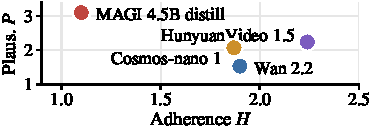
\includegraphics[width=\linewidth,
            height=\dimexpr\dp\PLtab-\dp\PLcap\relax]{fig/fig_mean_dotplot.pdf}\par\nointerlineskip
        \usebox{\PLcap}
    \end{minipage}
\end{figure}

The reverse also holds. Of the 28 videos that follow the stated property, 15 are rated implausible ($P \leq 2$): the model gets the property right but breaks other physics along the way. \textbf{Plausibility and grounding measure different things, and a benchmark has to measure both.}

\subsection{RQ2: Does Stating a Property in Text Reduce Plausibility?}
\label{sec:results-paired}

Each unobservable video has an observable twin: the same scene, action and generator, differing only in whether the property is shown in the image or stated in the text. Comparing twins, plausibility drops for every one of the four models when the property moves into the text, by 0.13 to 0.38 points on the 1--4 scale (Table~\ref{tab:paired-results}). Across all pairs, plausibility falls in 40 and rises in only 26.

% Table 5 and Figure 5 side by side, heights matched as for Table 4 / Figure 4.
\begin{figure}[t]
    \centering
    \sbox{\PLtab}{\begin{minipage}[t]{0.485\linewidth}
        \vspace{0pt}
        \centering
        \setlength{\abovecaptionskip}{0pt}
        \captionof{table}{Matched plausibility comparison. Obs., Unobs.: mean $P$ on the matched pairs; $\Delta$: unobservable minus observable. $p$: Holm-adjusted paired test; pooled row: scenario-level sign-flip test over the 29 scenarios annotated for all four models.}
        \label{tab:paired-results}
        \footnotesize
        \setlength{\tabcolsep}{3pt}
        \resizebox{\linewidth}{!}{%
        \begin{tabular}{@{}lrrrrr@{}}
            \toprule
            Model & $n$ & Obs. & Unobs. & $\Delta$ & $p$ \\
            \midrule
            HunyuanVideo 1.5  & 29 & 2.62 & 2.24 & $-0.38$ & 0.709 \\
            MAGI 4.5B distill & 30 & 3.33 & 3.10 & $-0.23$ & 0.884 \\
            Wan 2.2           & 30 & 1.83 & 1.53 & $-0.30$ & 0.497 \\
            Cosmos-nano 1     & 30 & 2.20 & 2.07 & $-0.13$ & 0.884 \\
            \midrule
            Pooled            & 29 & ---  & ---  & $-0.28$ & 0.085 \\
            \bottomrule
        \end{tabular}}
    \end{minipage}}%
    \sbox{\PLcap}{\begin{minipage}[t]{0.485\linewidth}
        \vspace{0pt}
        \setlength{\abovecaptionskip}{4pt}
        \captionof{figure}{Paired change $\Delta = P^{\mathrm{unobs}} - P^{\mathrm{obs}}$ per model and pooled, with bootstrap intervals over scenarios.}
        \label{fig:paired-effects}
    \end{minipage}}%
    \usebox{\PLtab}\hfill
    \begin{minipage}[t]{0.485\linewidth}
        \vspace{0pt}
        \centering
        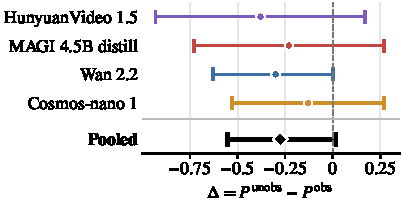
\includegraphics[width=\linewidth,
            height=\dimexpr\dp\PLtab-\dp\PLcap\relax]{fig/fig_forest_plausibility.pdf}\par\nointerlineskip
        \usebox{\PLcap}
    \end{minipage}
\end{figure}

Pooling the 29 scenarios that all four models generated gives the same picture: plausibility falls by 0.28 points on average (Figure~\ref{fig:paired-effects}; $p = 0.085$), and every model's estimate lies below zero. \textbf{Models produce less convincing physics when they have to read a property rather than see it.}

\subsection{RQ3: What Do Failure Cases Reveal About Grounding and Plausibility?}
\label{sec:results-cases}

\begin{figure}[t]
    \centering
    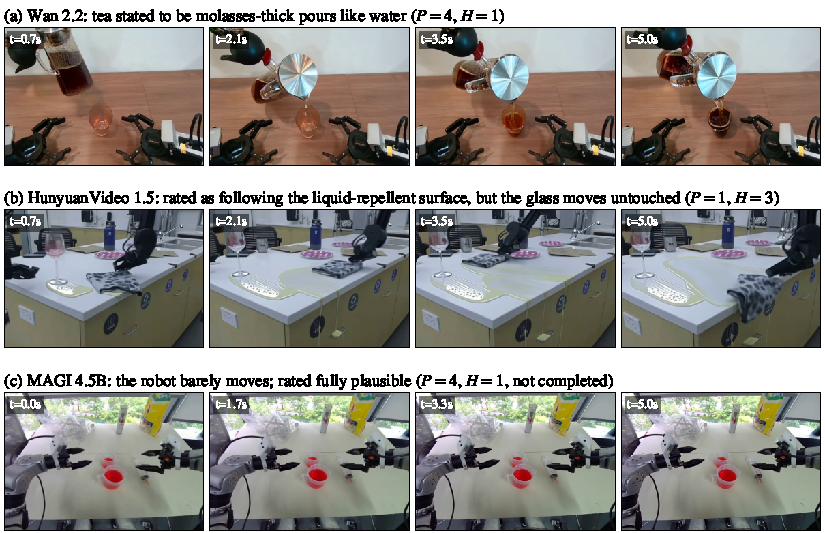
\includegraphics[width=\linewidth]{fig/fig_failure_cases.pdf}
    \caption{Three annotated failure cases (four frames each). $P$: physical plausibility; $H$: hidden-property adherence (both 1--4). (a) A clean, realistic pour that ignores the stated viscosity. (b) A video rated as following the stated property that is nevertheless physically implausible. (c) A nearly static video rated fully plausible.}
    \label{fig:failure-cases}
\end{figure}

Individual videos show how plausibility and grounding come apart (Figure~\ref{fig:failure-cases}; quotes are from the annotators' notes). In scenario 019, the prompt describes the tea as ``molasses-like'', yet all four models pour it like water ($H{=}1$) in videos rated realistic, and Wan~2.2 (Figure~\ref{fig:failure-cases}a) even receives the top plausibility rating: the models follow what the teapot looks like, not what the text says. The reverse also happens. In scenario 022, HunyuanVideo~1.5 follows the stated silicone-coated table ($H{=}3$) but is rated least plausible because of ``the glass moving without being touched'' (Figure~\ref{fig:failure-cases}b), and in scenario 070, Wan~2.2 keeps an ``extremely heavy'' tape dispenser still only because ``the robot's hand passes through it'' ($P{=}1$). MAGI's high plausibility often comes from inaction: in scenario 011 (Figure~\ref{fig:failure-cases}c) the robot barely moves, so nothing breaks physics because nothing happens. PhysicsLENS catches the visible failures, ranking HunyuanVideo's moving glass among the four least plausible of 433 videos and naming it a fluid violation with probability 0.997, as the annotators did, whereas the ignored viscosity in scenario 019 leaves nothing visibly wrong for any plausibility judge to catch. \textbf{Grounding has to be tested directly, and the matched design of PhysicsLENS makes that possible.}

\subsection{RQ4: Can PhysicsLENS Approximate Human Judgments?}
\label{sec:results-tool}

Can PhysicsLENS stand in for human annotators? We run its stages on all 439 annotated videos and compare the results with the human ratings, using ten open-weight VLMs from seven families (7B--32B parameters; Qwen3-VL, Qwen2.5-VL, InternVL3, Gemma-3, Llama-4-Scout, LLaVA-OneVision and Mistral-Small-3.1) and VideoPhy-2~\citep{bansal2026videophy} as an independent check. Each VLM answer is read as a probability; VLM answers and Stage-1/2 signals are combined with a weight fitted on the training folds, and any signal selection uses five-fold cross-validation that keeps every version of a scenario in the same fold, so nothing is tuned on the videos it is tested on. We report AUC: the probability that a better-rated video receives the higher score (0.5 is chance, 1 is perfect). Appendix~\ref{app:additional-results} gives the stage-by-stage results and agreement on the annotators' own scale.

\textbf{PhysicsLENS is the strongest evaluator.} Table~\ref{tab:main-results} compares PhysicsLENS with two baselines and with single VLM judges. The full system, which asks every question of all ten VLMs, averages their answers and combines them with the Stage-1/2 signals, is the best or tied-best system on six of the seven measures: plausibility (0.72 overall), task completion (0.81), violation detection (0.73), physics family (0.62) and property adherence (0.71). Even with a single VLM, adding PhysicsLENS evidence helps across the board: averaged over the ten VLMs, plausibility rises from 0.53 to 0.61, violation detection from 0.58 to 0.72, task completion from 0.71 to 0.76 and property adherence from 0.57 to 0.70, and detection and adherence improve for every one of the ten. The signals alone, with no VLM, already reach 0.70 on violation detection; the one selected most often measures objects vanishing mid-frame, a violation read directly off the tracker. The strongest baseline scores each video by its generator's average rating, which works because the four generators differ widely in quality. It ties PhysicsLENS on unobservable videos (0.72 vs.\ 0.71), but it cannot tell a good video from a bad one made by the same model: within each generator it scores 0.5 by construction, while PhysicsLENS reaches 0.67 on unobservable plausibility and 0.76 on task completion. It also does not exist for a new generator, which is exactly where an automatic evaluator is needed.

\begin{table*}[t]
    \centering
    \small
    \setlength{\tabcolsep}{2.4pt}
    \begin{tabular}{@{}lccc|cccc@{}}
        \toprule
        & \multicolumn{3}{c|}{Physical plausibility} & Task & Violation & Constr. & Hidden \\
        System & Obs. & Unobs. & All & compl. & detection & family & property \\
        \midrule
        \multicolumn{8}{@{}l}{\emph{Baselines}} \\
        Generator identity & 0.63{\scriptsize$\pm$0.03} & \textbf{0.72{\scriptsize$\pm$0.05}} & 0.65{\scriptsize$\pm$0.03} & 0.72{\scriptsize$\pm$0.02} & \textbf{0.73{\scriptsize$\pm$0.03}} & 0.51{\scriptsize$\pm$0.02} & 0.68{\scriptsize$\pm$0.05} \\
        Signals only (no VLM) & 0.61{\scriptsize$\pm$0.03} & 0.65{\scriptsize$\pm$0.05} & 0.62{\scriptsize$\pm$0.03} & 0.70{\scriptsize$\pm$0.03} & 0.70{\scriptsize$\pm$0.03} & 0.51{\scriptsize$\pm$0.02} & 0.69{\scriptsize$\pm$0.05} \\
        \midrule
        \multicolumn{8}{@{}l}{\emph{One VLM (mean $\pm$ sd over 10 backbones)}} \\
        VLM only & 0.53{\scriptsize$\pm$0.06} & 0.53{\scriptsize$\pm$0.06} & 0.53{\scriptsize$\pm$0.05} & 0.71{\scriptsize$\pm$0.04} & 0.58{\scriptsize$\pm$0.08} & 0.59{\scriptsize$\pm$0.02} & 0.57{\scriptsize$\pm$0.03} \\
        VLM + signals & 0.60{\scriptsize$\pm$0.02} & 0.66{\scriptsize$\pm$0.01} & 0.61{\scriptsize$\pm$0.01} & 0.76{\scriptsize$\pm$0.02} & 0.72{\scriptsize$\pm$0.01} & 0.58{\scriptsize$\pm$0.02} & 0.70{\scriptsize$\pm$0.02} \\
        Debiased VLM & 0.64{\scriptsize$\pm$0.07} & 0.63{\scriptsize$\pm$0.04} & 0.63{\scriptsize$\pm$0.06} & 0.71{\scriptsize$\pm$0.04} & 0.58{\scriptsize$\pm$0.08} & 0.59{\scriptsize$\pm$0.02} & 0.57{\scriptsize$\pm$0.03} \\
        Debiased VLM + signals & 0.65{\scriptsize$\pm$0.05} & 0.67{\scriptsize$\pm$0.03} & 0.65{\scriptsize$\pm$0.04} & 0.76{\scriptsize$\pm$0.02} & 0.72{\scriptsize$\pm$0.01} & 0.58{\scriptsize$\pm$0.02} & 0.70{\scriptsize$\pm$0.02} \\
        \midrule
        \multicolumn{8}{@{}l}{\emph{PhysicsLENS with all ten VLMs}} \\
        Ensemble, debiased & \textbf{0.73{\scriptsize$\pm$0.03}} & 0.71{\scriptsize$\pm$0.05} & \textbf{0.72{\scriptsize$\pm$0.02}} & 0.77{\scriptsize$\pm$0.02} & 0.67{\scriptsize$\pm$0.03} & \textbf{0.63{\scriptsize$\pm$0.01}} & 0.59{\scriptsize$\pm$0.06} \\
        Ensemble + signals (full) & \textbf{0.73{\scriptsize$\pm$0.03}} & 0.71{\scriptsize$\pm$0.05} & \textbf{0.72{\scriptsize$\pm$0.02}} & \textbf{0.81{\scriptsize$\pm$0.02}} & \textbf{0.73{\scriptsize$\pm$0.03}} & 0.62{\scriptsize$\pm$0.02} & \textbf{0.71{\scriptsize$\pm$0.05}} \\
        \bottomrule
    \end{tabular}
    \caption{PhysicsLENS against human judgment (AUC; 439 videos). \emph{Plausibility}: human rating 3--4 vs.\ 1--2. \emph{Task compl.}: completed vs.\ not. \emph{Violation detection}: any recorded violation vs.\ none. \emph{Constr.\ family}: naming which physics family was violated. \emph{Hidden property}: whether the stated property was followed (unobservable videos). \emph{Signals}: PhysicsLENS Stage-1/2 measurements, combined with the VLM answers using a weight fitted on training folds; the full system also includes temporal-embedding signals. \emph{Debiased}: the PhysicsLENS physics-error question, which replaces only the plausibility question. \emph{Ensemble}: every question asked of all ten VLMs and their answers averaged by rank, with no backbone selected. \emph{Generator identity} scores each video by its generator's average on the training folds. $\pm$: sd across the ten VLMs for the one-VLM rows, bootstrap sd over videos otherwise. Bold: best in each column.}
    \label{tab:main-results}
\end{table*}

\textbf{Why a VLM alone falls short.} Asked plainly whether a video is physically plausible, most VLMs do little better than chance (AUC 0.45--0.63; Table~\ref{tab:backbones-obs-unobs}). Shown two videos of the same task, they even pick the less realistic one more often than not (Gemma-3-12B is right in only 36\% of 347 pairs), because they favor the video with more motion and more task progress: VLMs treat \emph{plausible} as \emph{successful}, the same trap MAGI's near-static videos expose from the human side (Section~\ref{sec:results-cases}).

\textbf{Asking about physics errors, not overall realism.} The PhysicsLENS screening question instead asks the VLM to count specific physics errors (objects passing through each other, appearing or vanishing, floating, changing shape impossibly, or moving untouched) and to ignore task success and the amount of motion; the tables call it the \emph{debiased} question. This one change improves eight of the ten VLMs, the best by 0.20 (Qwen3-VL-32B: 0.55 to 0.75; InternVL3-14B: 0.51 to 0.71). It carries over to VideoPhy-2, a benchmark it was not designed for, where it significantly improves all three VLMs we tested (Qwen3-VL-32B: 0.645 to 0.720). It also lets bigger models pull ahead: with the plain question the 14B and 32B models trail their 7B and 8B counterparts, and with the PhysicsLENS question they lead them.

\begin{table}[t]
    \centering
    \small
    \setlength{\tabcolsep}{3.5pt}
    \begin{tabular}{@{}lcccccc|c@{}}
        \toprule
        & \multicolumn{2}{c}{VLM, standard prompt} & \multicolumn{2}{c}{VLM, debiased} & \multicolumn{2}{c|}{Debiased + S1/2} & Hidden \\
        \cmidrule(lr){2-3}\cmidrule(lr){4-5}\cmidrule(lr){6-7}
        Backbone & Obs. & Unobs. & Obs. & Unobs. & Obs. & Unobs. & AUC \\
        \midrule
        Signals only (S1/2) & --- & --- & --- & --- & 0.61 & 0.65 & 0.69 \\
        Qwen3-VL-32B & 0.55 & 0.55 & 0.75 & 0.70 & 0.74 & 0.70 & 0.57 \\
        InternVL3-14B & 0.51 & 0.45 & 0.71 & 0.65 & 0.71 & 0.68 & 0.51 \\
        Qwen3-VL-8B & 0.54 & 0.58 & 0.68 & 0.69 & 0.68 & 0.71 & 0.56 \\
        Qwen2.5-VL-32B & 0.45 & 0.44 & 0.66 & 0.64 & 0.67 & 0.71 & 0.57 \\
        InternVL3-8B & 0.63 & 0.62 & 0.66 & 0.59 & 0.65 & 0.61 & 0.59 \\
        Llama-4-Scout-17B & 0.58 & 0.48 & 0.64 & 0.61 & 0.64 & 0.65 & 0.59 \\
        Qwen2.5-VL-7B & 0.45 & 0.54 & 0.61 & 0.64 & 0.63 & 0.67 & 0.55 \\
        Gemma-3-12B & 0.61 & 0.61 & 0.59 & 0.59 & 0.60 & 0.65 & 0.56 \\
        LLaVA-OV-7B & 0.47 & 0.54 & 0.54 & 0.62 & 0.59 & 0.66 & 0.61 \\
        Mistral-Small-3.1-24B & 0.53 & 0.54 & 0.53 & 0.58 & 0.58 & 0.66 & 0.56 \\
        \bottomrule
    \end{tabular}
    \caption{Plausibility AUC for each VLM on observable ($n{=}320$) and unobservable ($n{=}119$) videos: with a standard question, with the PhysicsLENS physics-error (debiased) question, and with that question combined with Stage-1/2 signals (S1/2). \emph{Hidden}: AUC for judging whether the stated property was followed.}
    \label{tab:backbones-obs-unobs}
\end{table}

\textbf{Observable versus unobservable videos.} PhysicsLENS judges plausibility almost as well when the property is stated in text as when it is visible (Qwen3-VL-32B: 0.70 vs.\ 0.75). Judging whether the stated property was actually followed is harder, and this is where the signals help most, raising AUC from 0.51--0.61 for VLMs alone to 0.70 on average and 0.74 at best.

\textbf{Which kind of physics failed.} PhysicsLENS reliably detects each of the seven kinds of violation, separating affected videos from clean ones with AUC 0.66--0.84, and the signals improve this for six of the seven (Table~\ref{tab:category-accuracy}). Naming the exact family among several violations is harder, except for fluids (0.82): most violating videos (69\%) break several kinds of physics at once, and VLMs read frames largely one at a time, which suits single-frame failures such as a splash better than failures over time such as gravity or friction. Failures over time are exactly what the tracking-based measurements of the Stage-3 specialists are built for.

\begin{table}[t]
    \centering
    \small
    \setlength{\tabcolsep}{4pt}
    \begin{tabular}{@{}lrccc|cc@{}}
        \toprule
        & & \multicolumn{3}{c|}{Attribution AUC} & \multicolumn{2}{c}{Detection AUC} \\
        Constraint family & Pos. & Best VLM & Mean$\pm$sd (10) & Signals & Best VLM & +S1/2 \\
        \midrule
        Collision & 167 & 0.57 {\scriptsize Q3-32B} & 0.54$\pm$0.02 & 0.45 & 0.67 {\scriptsize Q3-32B} & 0.73 \\
        Deformation & 146 & 0.61 {\scriptsize G3-12B} & 0.58$\pm$0.03 & 0.60 & 0.68 {\scriptsize Q2.5-7B} & 0.74 \\
        Causality & 169 & 0.59 {\scriptsize Q3-32B} & 0.54$\pm$0.03 & 0.53 & 0.56 {\scriptsize Q3-8B} & 0.69 \\
        Momentum & 59 & 0.58 {\scriptsize Q2.5-7B} & 0.53$\pm$0.04 & 0.46 & 0.67 {\scriptsize Q3-8B} & 0.67 \\
        Gravity & 44 & 0.66 {\scriptsize Q2.5-7B} & 0.55$\pm$0.08 & 0.56 & 0.72 {\scriptsize Q3-8B} & 0.75 \\
        Fluid & 35 & 0.87 {\scriptsize Q2.5-7B} & 0.82$\pm$0.03 & 0.53 & 0.84 {\scriptsize Q2.5-7B} & 0.80 \\
        Friction & 24 & 0.65 {\scriptsize Q3-32B} & 0.57$\pm$0.05 & 0.48 & 0.66 {\scriptsize IV-14B} & 0.69 \\
        \bottomrule
    \end{tabular}
    \caption{Accuracy by physics family (AUC). \emph{Detection}: videos with this family vs.\ the 106 videos with no violation. \emph{Attribution}: videos with this family vs.\ videos with a different violation (Contact merged into Collision). \emph{Pos.}: videos with this family. \emph{Best VLM} is the best of ten; \emph{Mean$\pm$sd} is over all ten. Q3 = Qwen3-VL, Q2.5 = Qwen2.5-VL, IV = InternVL3, G3 = Gemma-3.}
    \label{tab:category-accuracy}
\end{table}



\section{Conclusion}

We introduced PhysicsLENS, a benchmark and diagnostic pipeline for physical grounding in generated robot video. Its matched scenarios hold the conditioning frame and the action fixed and change only whether a governing physical property is visible in the image or stated in the text. Across four video generation models and 439 human-annotated videos, this design exposes a failure that plausibility scores cannot see: 72\% of the unobservable videos rated realistic ignore the stated property, and every model loses plausibility when a property must be read rather than seen. Current video generators therefore do not treat physical realism and property grounding as one capability, and a benchmark that measures realism alone cannot tell a model that reasons about stated physics from one that animates what the image looks like.

PhysicsLENS also makes this evaluation automatic. Asking vision-language models about specific physics errors rather than overall realism, and grounding their answers in measured tracking and motion signals, turns off-the-shelf judges that mostly reward task success into evaluators that track human judgment. The full pipeline is the best or tied-best system on six of seven measures, reaching 0.72 AUC on plausibility and 0.81 on task completion, and it separates good from bad videos within each generator, where shortcuts based on the generator's identity fail. As video world models are increasingly used as training environments for robots, whether a model follows the physics it is given, not only whether its output looks right, decides whether those environments can be trusted. PhysicsLENS provides the matched data and the automatic diagnosis needed to measure exactly that.

\section{Limitations and Future Work}

Although PhysicsLENS provides a novel contribution to physics-benchmarks for video generation, we acknowledge current limitations. These include having a single-annotator pass for video annotations, and the limitation of generated videos per model. Future work includes collecting overlapping annotations to establish inter-annotator reliability, expanding the matched scenario set to increase statistical power, and extending the rubric to separately encode contradiction versus non-demonstration of a stated property.

\section{AI Use Statement}
In this work, we used generative AI tools for: drafting portions of the final text, generating code for the diagnostic tool and annotation pipeline. We have not used generative AI tools for: generating experimental results or designing core methodology.
We have reviewed all AI-assisted work. We take responsibility for the final content of this work, including text, claims, or artifacts produced with the aid of generative AI.

\section{Ethics Statement}
This work aligns with the ICLR Code of Ethics as it does not involve human subjects or sensitive information. All datasets used are publicly available and licensed for research use. We ensured that all results and methods are explained accurately, transparently, and reproducibly. Our work aligns with responsible and beneficial use of video-generation improvement for robotics.

\section{Reproducibility Statement}
\Isaiah{Not part of the 9 page limit}

\bibliography{iclr2026_conference}
\bibliographystyle{iclr2027_conference}

\clearpage
\appendix
\section{Dataset Details}
\label{app:dataset-details}

\subsection{Image and Prompt Preparation}
Source frames were captured or collected at, or upscaled to, $1280\times720$ (16:9). Frames below this resolution were padded to a 16:9 aspect ratio when necessary and upscaled with bicubic interpolation rather than generative enhancement. Each frame depicts the scene immediately before the relevant action begins, never mid-action, so that the conditioning image specifies the initial state.

A vision-language model generated scene and action descriptions under a fixed annotation schema, after which the descriptions were reviewed for accuracy. Every rendered prompt appends a fixed instruction specifying a static, fixed-viewpoint camera without panning, zooming, or motion. This constraint reduces the risk that camera movement is misattributed to object physics during evaluation.

\subsection{Taxonomy and curation notes}
Collision and Friction scenarios were comparatively easy to source, reflecting the prevalence of pick-and-place and surface-manipulation footage. Fluid and Deformation scenarios were harder to find, while Gravity scenarios that isolated free fall were rare outside incidental object drops. Table~\ref{tab:dataset-stats} reports the resulting domain distribution. These observations describe our curation process only; establishing the distribution of public robotics video would require a systematic survey of available sources.

\paragraph{Annotation procedure.} Scenarios were curated from public robotics video sources rather than authored domain-first, and each scenario was subsequently annotated with its governing physical domain by manual review of its action and outcome. This annotation was performed independently of the taxonomy's construction to avoid circularity: the seven domains were fixed in advance from the specialist families, and each scenario was assigned to the domain its physics most directly tests, rather than domains being defined post hoc to fit whatever scenarios happened to be available.

\paragraph{Interaction with observability.} The observable/unobservable axis introduced in \S\ref{sec:observability} is orthogonal to domain: a scenario's domain label is fixed by the physical law under test, while its observability condition determines whether the property governing that law is visually apparent or text-specified. Both matched members of an observable/unobservable pair therefore carry the same domain label, allowing the accuracy gap described in \S\ref{sec:observability} to be reported per domain rather than only in aggregate.

\section{Human annotation}
\subsection{Human Annotation Rubrics}
\label{app:annotation-details}

\paragraph{Physical plausibility.}
Each video receives a physical-plausibility rating $P\in\{1,2,3,4\}$ based on visible contact, motion, deformation, and object persistence:
\begin{enumerate}
    \item \textbf{Clearly breaks physics:} clipping, floating, object appearance or disappearance, or impossible motion.
    \item \textbf{Mostly implausible:} one clear issue or several smaller issues.
    \item \textbf{Mostly plausible:} minor oddities only.
    \item \textbf{Physically realistic:} the interaction looks real.
\end{enumerate}
These scores are human judgments of visible behavior, not measurements of agreement with a physical simulator.

\paragraph{Hidden-property adherence.}
For unobservable scenarios, annotators receive a question identifying the stated property and asking whether it is reflected in the generated behavior. Adherence is rated as $H\in\{1,2,3,4\}$:
\begin{enumerate}
    \item \textbf{Completely ignored:} the outcome shows no indication of the stated property.
    \item \textbf{Mostly ignored:} the property is indicated only faintly or inconsistently.
    \item \textbf{Mostly followed:} the property is reflected, but with incorrect magnitude, timing, or degree.
    \item \textbf{Fully followed:} the property is fully and correctly reflected in the outcome.
\end{enumerate}
Adherence is not rated for observable scenarios, and missing adherence values are not treated as zero or as failures. The rubric does not separately encode a visible contradiction of the property and a failure to perform the interaction needed to reveal it; we retain this distinction when interpreting low scores.

\paragraph{Action completion.}
Annotators answer the binary question, ``Is the task done by the end, even if the physics looked wrong?'' We encode this response as $A\in\{0,1\}$. Completion is evaluated separately because a video may finish the action through implausible behavior or depict plausible behavior without completing the task.

\paragraph{Issue descriptions and violation labels.}
The annotation form requests a short description of the physical issue and permits multiple labels: Causality, Collision, Contact, Deformation, Fluid, Friction, Gravity, and Momentum. Although annotators select the most obvious issue first and the export preserves this order, our frequency analysis treats the labels as an unordered set. Selection order is not interpreted as severity.

These eight annotation labels differ from the seven physical families used to organize the benchmark and its specialists. In particular, Contact and Collision remain separate in the human-label analyses rather than being merged through an undocumented mapping. A blank category field means that no violation label was recorded, not that the video was independently verified as physically correct.

\paragraph{Annotator background and allocation.}
Annotators were master's students, PhD candidates, and PhD holders from a computer science research environment. Videos were randomly allocated without conditioning on model or scenario. For HunyuanVideo, MAGI, and Wan, observable annotations were assigned in groups of 16--17 videos per annotator. Unobservable annotations were assigned in groups of six, except for one group of five for HunyuanVideo. Observable Cosmos records used a different allocation and include a combined annotator label.

Each clip received one annotation rather than independent ratings from multiple annotators, so inter-annotator reliability cannot be estimated. In 99 of the 119 available video-level matched pairs, the recorded annotator labels differ between conditions. Paired analyses therefore control for scenario identity but not for differences in annotator calibration.

\paragraph{Aggregation.}
We report rating distributions, descriptive means of the ordinal scores, and action-completion proportions. We interpret $P\geq3$ as mostly plausible or physically realistic and $H\geq3$ as mostly or fully adhering to the specified property. We also examine the joint distribution of $P$ and $H$, including the proportion of videos with $H\leq2$ among those with $P\geq3$. These dimensions are reported separately rather than combined into a single score.
\section{Additional Results}
\label{app:additional-results}
Table~\ref{tab:stage-ablation} adds the PhysicsLENS stages one at a time. For violation detection, every stage adds evidence: the Stage-1 and Stage-2 signals improve every VLM (e.g.\ InternVL3-8B: 0.67 to 0.72; Gemma-3-12B: 0.65 to 0.71). For plausibility, the signals bring weaker VLMs up toward the strongest; on top of Qwen3-VL-32B with the PhysicsLENS question they add little, because their main contribution, object speed, is the activity cue that the question already corrects for. Table~\ref{tab:pipeline-human-agreement} reports agreement with the annotators on their own 1--4 scale: $\kappa_w{=}0.32$ for plausibility, $\kappa{=}0.38$ for task completion and $\kappa_w{=}0.21$ for property adherence.

\begin{table}[h]
    \centering
    \small
    \setlength{\tabcolsep}{5pt}
    \begin{tabular}{@{}lcccc|cccc@{}}
        \toprule
        & \multicolumn{4}{c|}{Violation detection (AUC)} & \multicolumn{4}{c}{Plausibility (AUC)} \\
        MLLM backbone & VLM & S1 & S1+2 & Full tool & VLM & S1 & S1+2 & Full tool \\
        \midrule
        No VLM (signals only) & --- & 0.68 & 0.70 & --- & --- & 0.58 & 0.62 & --- \\
        Qwen3-VL-32B & 0.74 & 0.75 & 0.76 & 0.75 & 0.74 & 0.69 & 0.71 & 0.72 \\
        Qwen3-VL-8B & 0.74 & 0.74 & 0.75 & 0.76 & 0.69 & 0.66 & 0.67 & 0.68 \\
        InternVL3-14B & 0.66 & 0.70 & 0.72 & 0.71 & 0.69 & 0.66 & 0.69 & 0.70 \\
        InternVL3-8B & 0.67 & 0.71 & 0.72 & 0.68 & 0.64 & 0.63 & 0.65 & 0.62 \\
        Gemma-3-12B & 0.65 & 0.70 & 0.71 & 0.73 & 0.59 & 0.60 & 0.62 & 0.62 \\
        Qwen2.5-VL-7B & 0.70 & 0.73 & 0.75 & 0.73 & 0.62 & 0.62 & 0.64 & 0.63 \\
        \bottomrule
    \end{tabular}
    \caption{Cumulative stage ablation on the 439 annotated clips. \emph{VLM}: the backbone's debiased screening question alone. \emph{S1}: fused with Stage-1 screening signals (frame differences, optical flow, camera motion). \emph{S1+2}: additionally Stage-2 track kinematics (camera-compensated Lucas--Kanade tracks, track loss, per-object speed and acceleration). \emph{Full tool}: additionally the Stage-3 specialist judgment ($1-P(\text{no violation})$ from a single forced-choice query over the seven constraint families). Numeric signals are selected and oriented on training folds only; channels are combined by an unweighted rank mean. Violation detection separates clips with any human-recorded violation ($n{=}333$) from clips with none ($n{=}106$). Stage~4 organizes and
      summarizes findings but contributes no additional score, so the full tool
      is Stages~1--3.}
    \label{tab:stage-ablation}
\end{table}

\begin{table}[h]
    \centering
    \small
    \setlength{\tabcolsep}{4pt}
    \begin{tabular}{@{}lrcccccc@{}}
        \toprule
        & & \multicolumn{2}{c}{Plausibility} & \multicolumn{2}{c}{Hidden property} & \multicolumn{2}{c}{Completion} \\
        \cmidrule(lr){3-4}\cmidrule(lr){5-6}\cmidrule(lr){7-8}
        Generator & $n$ & $\kappa_w$ & AUC & $\kappa_w$ & AUC & $\kappa$ & AUC \\
        \midrule
        Wan 2.2 & 110 & 0.18 & 0.73 & 0.18 & 0.64 & 0.21 & 0.69 \\
        Cosmos-nano 1 & 110 & 0.29 & 0.70 & 0.03 & 0.51 & 0.27 & 0.70 \\
        HunyuanVideo 1.5 & 109 & 0.10 & 0.58 & 0.02 & 0.63 & 0.17 & 0.65 \\
        MAGI 4.5B distill & 110 & 0.36 & 0.78 & 0.44 & --- & -0.02 & 0.90 \\
        \midrule
        Overall & 439 & 0.32 & 0.74 & 0.21 & 0.71 & 0.38 & 0.79 \\
        \bottomrule
    \end{tabular}
    \caption{Agreement between automated diagnosis and human annotation. Ratings are obtained from continuous scores by quantile matching fitted on training folds only (5-fold cross-validation grouped by task, so the observable and unobservable versions of a scenario never straddle a fold). $\kappa_w$ is linearly weighted Cohen's $\kappa$ on the 1--4 scale; completion uses unweighted $\kappa$. AUC separates ratings 3--4 from 1--2 (completion: yes vs.\ no). Plausibility: debiased Qwen3-VL-32B prompt; hidden property (unobservable clips only, $n{=}119$): Llama-4-Scout with the stated property plus Stage-1/2 signals; completion: Qwen3-VL-8B plus Stage-1/2 signals. Overall 95\% bootstrap CIs: plausibility [0.25, 0.39], hidden property [0.08, 0.35], completion [0.29, 0.47].}
    \label{tab:pipeline-human-agreement}
\end{table}

\section{PhysicsLENS diagnostic pipeline Details}
\label{app:pipeline-details}

The automated pipeline contains four stages---screening, localization, specialist evaluation, and reporting---supported by a shared evidence store containing tracks, masks, timestamps, measurements, and diagnostic findings. Routing depends on available evidence and the computational budget. The architecture defines the intended diagnostic process; it does not by itself establish diagnostic accuracy or cost savings.

\paragraph{Screening.}
The screening stage examines the generated video and its conditioning information to identify candidate physical inconsistencies and relevant constraint families. A screening flag is a candidate for further examination, not a verified violation.

\paragraph{Localization.}
The localization stage associates candidate issues with relevant temporal intervals and interacting objects, connecting each diagnosis to visible evidence rather than leaving it as a video-level assertion.

\paragraph{Specialist evaluation.}
Domain specialists assess candidate events against the physical constraints in Table~\ref{tab:specialists-scope}. Property-specific assessment uses the stated physical condition rather than assuming that a visually familiar object has its usual material properties. Specialist judgments also distinguish an observed inconsistency from insufficient visual evidence.

\paragraph{Reporting.}
The reporting stage organizes findings into a structured account of the implicated constraints, relevant events, and supporting observations. These stages specify intended functional roles and do not establish diagnostic accuracy.

\subsection{Domain-Specific Diagnostic Checks}
A single event may implicate multiple constraint families. Table~\ref{tab:specialists-scope} defines the intended scope of each specialist rather than claiming validated detector capabilities.

\begin{table}[t]
    \centering
    \small
    \caption{Intended scope of the seven PhysicsLENS specialists. Checks require visible evidence or an explicit property specification; they do not assume access to hidden forces, complete material parameters, or a reference outcome.}
    \label{tab:specialists-scope}
    \begin{tabular}{@{}p{0.16\linewidth}p{0.77\linewidth}@{}}
        \toprule
        Specialist & Diagnostic questions \\
        \midrule
        Collision & Do interactions respect object boundaries? Is apparent penetration inconsistent with object rigidity, and is motion attributed to contact supported by visible interaction? \\
        Friction & Is sticking, slipping, or sliding consistent with visible contact and any stated surface condition? Are changes in resistance supported by the interaction? \\
        Momentum & Are abrupt changes in translational or rotational motion supported by an interaction? Where mass is specified, does the video provide enough evidence to assess its consequences? \\
        Fluid & Is flow consistent with the visible container geometry and interaction? Are stated properties such as viscosity reflected when the action exposes them? \\
        Deformation & Do changes in shape follow the interaction and any stated material properties? Are apparent changes physical deformation or unsupported morphing? \\
        Gravity & Is unsupported motion consistent with gravity, accounting for visible support and contact? Is apparent floating distinguishable from unresolved support or perspective? \\
        Causality & Do object appearances, disappearances, and state changes have visible or otherwise supported causes? Could an apparent discontinuity instead result from occlusion? \\
        \bottomrule
    \end{tabular}
\end{table}

\subsection{Comparison with Human Judgments}
\label{app:pipeline-human-comparison}
The human ratings provide a reference for agreement, not error-free physical ground truth. Section~\ref{sec:pipeline-human-comparison} specifies the comparison and Section~\ref{sec:results-tool} reports it: AUC and linearly weighted Cohen's $\kappa$ for the ordinal ratings, AUC and Cohen's $\kappa$ for action completion, and per-family detection and attribution AUC for violations, with Contact merged into Collision. Hidden-property adherence is compared only on unobservable scenarios. Every fitted choice uses five-fold cross-validation grouped by scenario; the debiased judge prompt, written after inspecting these videos, is validated on VideoPhy-2.

The current annotations do not contain structured temporal boundaries or object-level ground truth. They therefore cannot establish localization accuracy, which would require additional annotation.

\subsection{Reference-Outcome-Free Diagnosis}
\label{app:ground-truth-free}
During inference, the pipeline does not receive \texttt{expected\_outcome}, a reference video, or human evaluation labels. Its permitted evidence comprises the generated video and conditioning information, including the initial image, requested action, and any text-specified physical property.

The stated property is part of the model input and is therefore available to the evaluator; this differs from providing a reference description of how the action should unfold. Human labels may be used afterward to measure agreement but are not supplied to the diagnostic stages. Because forces, material parameters, occluded contacts, and other quantities may remain unknown, diagnoses should be supported by available evidence and permit an insufficient-evidence outcome.


\end{document}
